\documentclass[a4paper]{article}

\usepackage[english]{babel}
\usepackage[T1]{fontenc}
\usepackage{amsmath}
\usepackage{graphicx}
\usepackage[colorinlistoftodos]{todonotes}
\usepackage{makeidx}
\usepackage{fullpage,xspace,setspace,lscape}
\makeindex

\renewcommand{\thefigure}{S\arabic{figure}}


\title{\huge\bfseries \vspace{2cm} The \textit{E. coli} molecular phenotype under different growth conditions \\ \vspace{0.7cm}
	\Large\bfseries Supplementary materials \vspace{1.3cm}}


\author{
	\large\bfseries Mehmet U. Caglar, John R. Houser, Craig S. Barnhart, \\
	\large\bfseries Daniel R. Boutz, Sean M. Carroll, Aurko Dasgupta, Walter F. Lenoir,\\ 
	\large\bfseries Bartram L. Smith, Viswanadham Sridhara, Dariya K. Sydykova, \\
	\large\bfseries Drew Vander Wood, Christopher J. Marx, \\
	\large\bfseries Edward M. Marcotte*, Jeffrey E. Barrick*, Claus O. Wilke*}


% allow floats to take up as much space as they want on a page
\renewcommand{\topfraction}{1.}	% max fraction of floats at top
\renewcommand{\bottomfraction}{1.}
\renewcommand{\textfraction}{0.}

\begin{document}
\maketitle
\newpage
	

\listoffigures


\newpage

\section*{Supplementary Figures}

\begin{figure}[!htb]
\centerline{	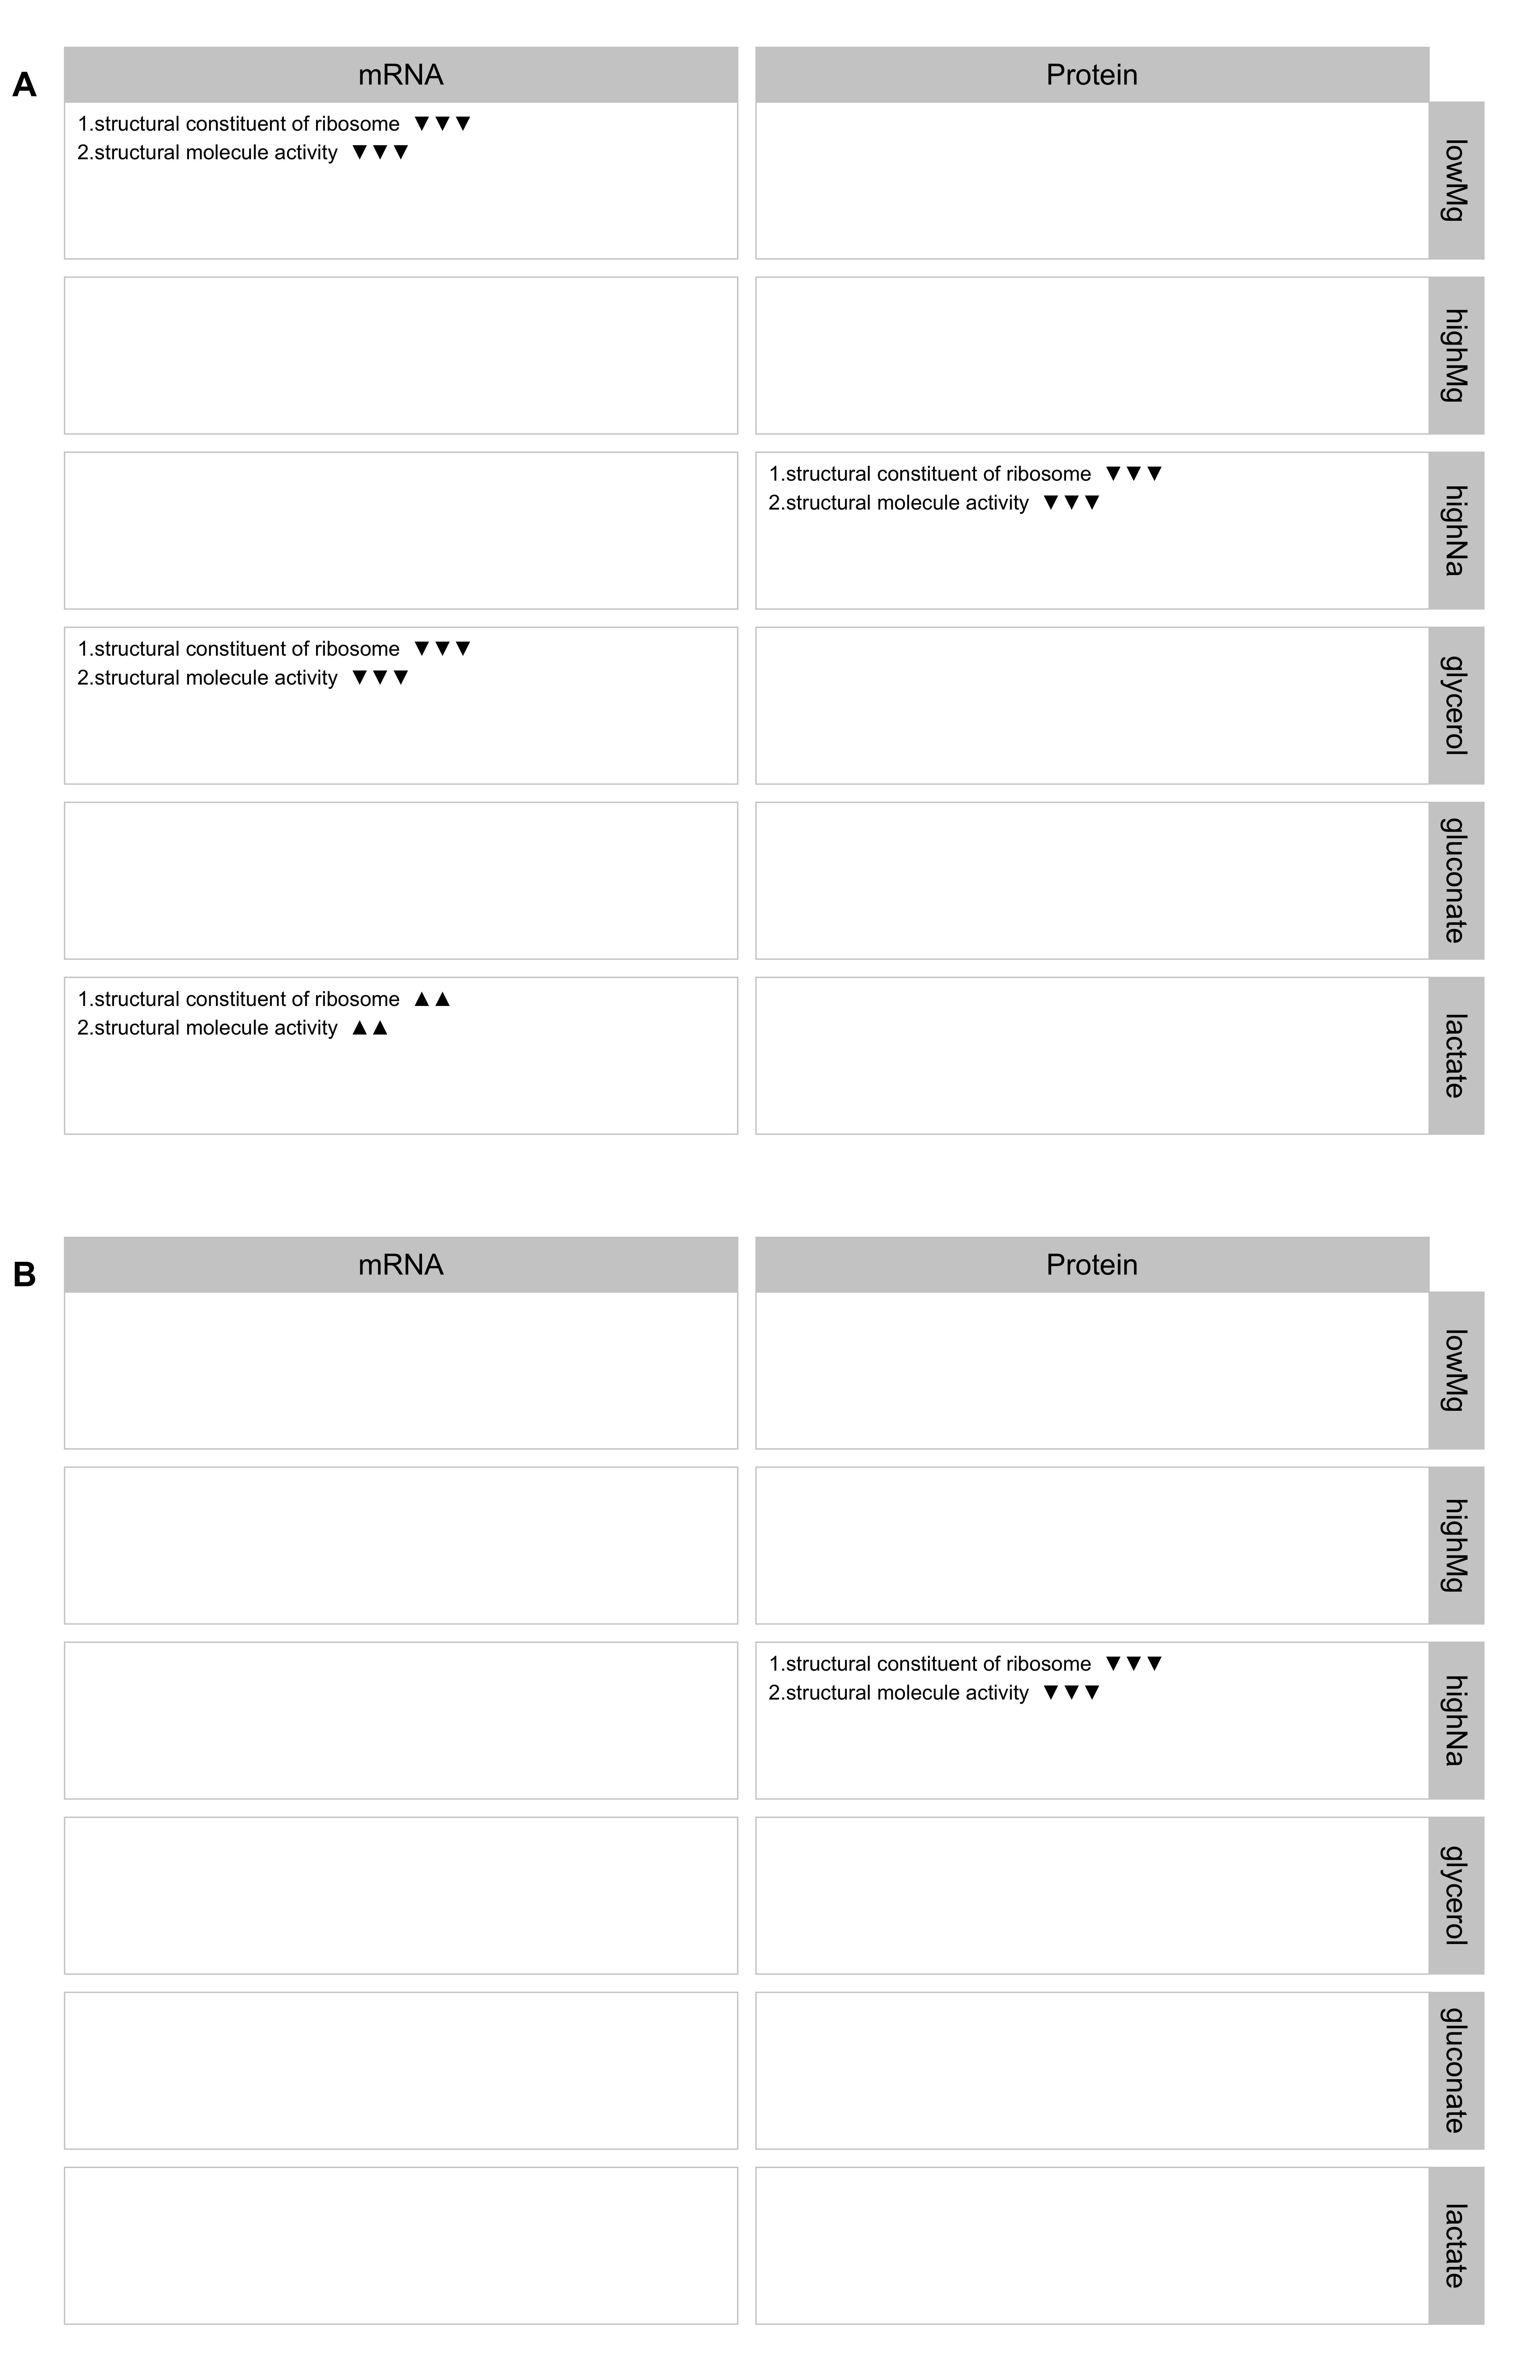
\includegraphics[width=0.7\textwidth]{../supplementary_figures/figS1_resultSummary_mf.png}
}
	\caption[Significantly differentially expressed molecular functions]
	{\textbf{Significantly differentially expressed molecular functions, as determined by GO annotations.} For each condition, we show the top-5 differentially expressed molecular functions according to either mRNA or protein abundances.  Empty boxes indicate that no differentially expressed pathways were found. The arrows next to pathway names indicate the proportion of up- and down-regulated genes among the significantly differentially expressed genes in this pathway. One up arrow indicates that 60\% or more of the genes are up-regulated, two arrows correspond to 80\% or more genes, and three arrows correspond to 95\% or more genes being up-regulated. Similarly, down arrows indicate the proportion of down-regulated genes. (A) Exponential phase. (B) Stationary phase.}
\end{figure}

\clearpage

\begin{figure}[!htb]
	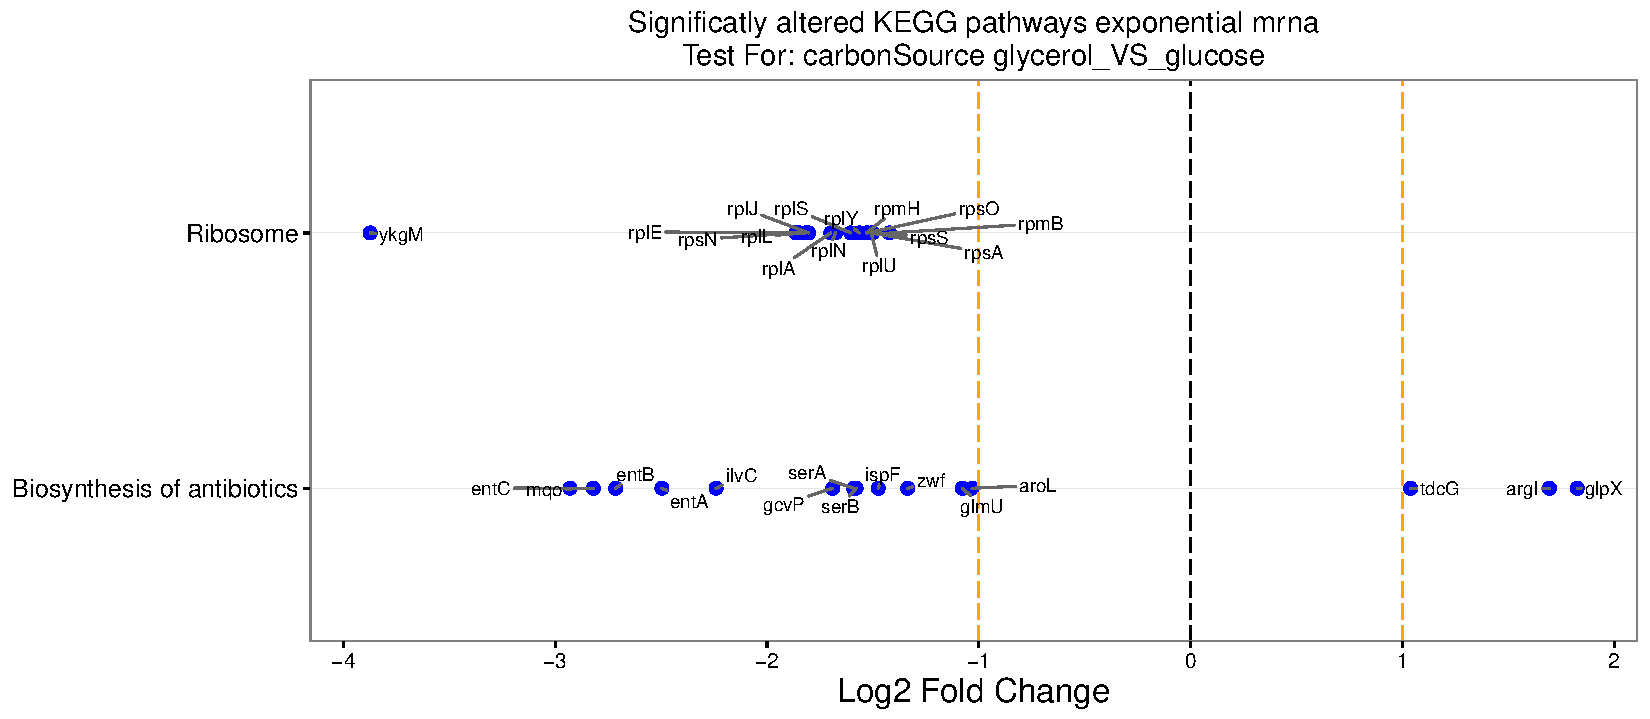
\includegraphics[width=1.0\textwidth]{../../d_figures/kegg_01.pdf}
	\caption[Significantly differentially expressed KEGG pathways for mRNA samples in exponential phase tested for glycerol against glucose]
	{\textbf{Significantly differentially expressed KEGG pathways and associated genes with glycerol as carbon source, as determined by mRNA abundances in exponential phase.} The top differentially expressed KEGG pathways are shown along the $y$ axis, and the relative fold change of the corresponding genes is shown along the $x$ axis. We show up to 10 of the most significantly changed pathways and for each pathway we show up to 15 of the most significantly changing genes.}
\end{figure}

\clearpage
\begin{figure}
	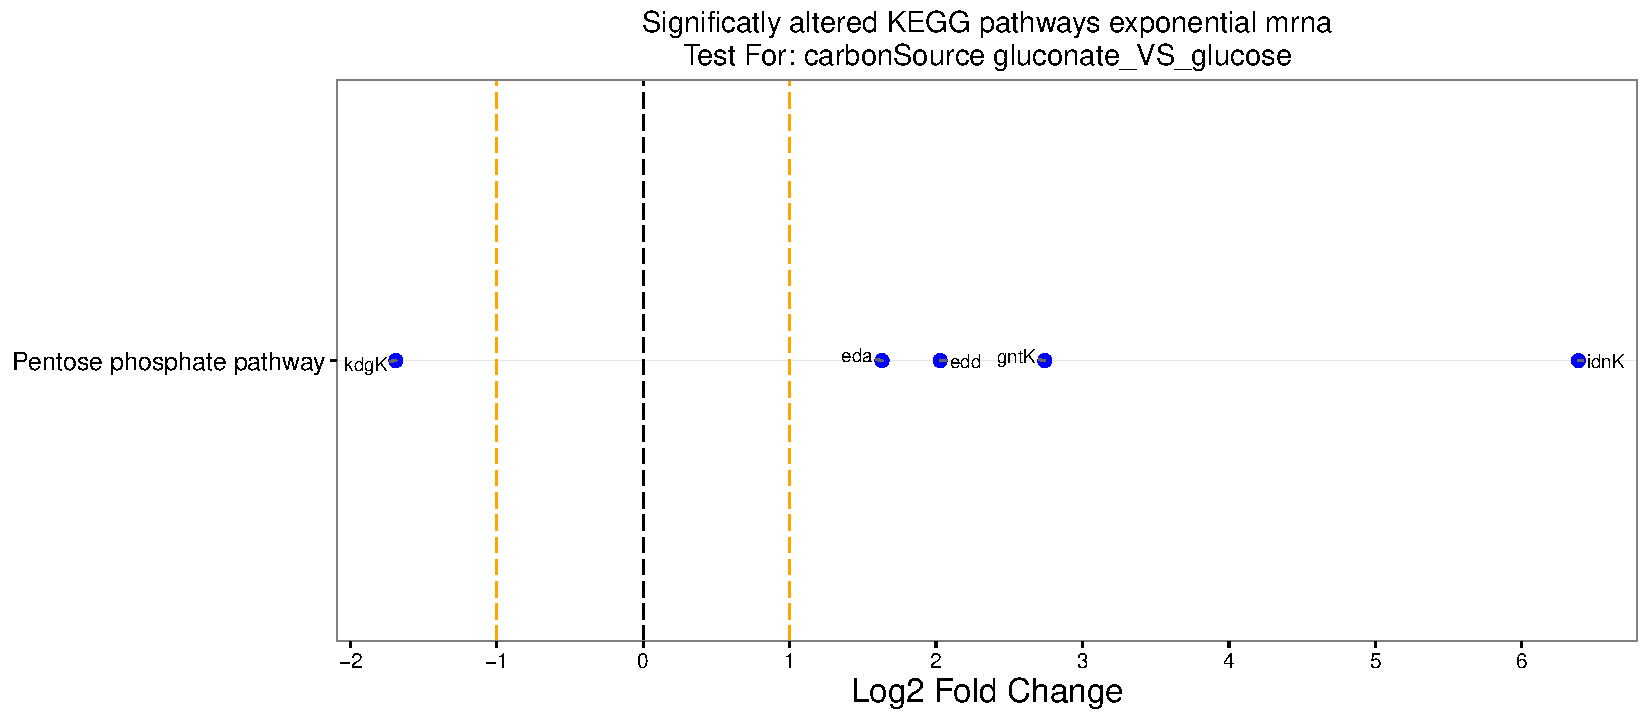
\includegraphics[width=1.0\textwidth]{../../d_figures/kegg_02.pdf}
	\caption[Significantly differentially expressed KEGG pathways for mRNA samples in exponential phase tested for gluconate against glucose]
	{\textbf{Significantly differentially expressed KEGG pathways and associated genes with gluconate as carbon source, as determined by mRNA abundances in exponential phase.} The top differentially expressed KEGG pathways are shown along the $y$ axis, and the relative fold change of the corresponding genes is shown along the $x$ axis. We show up to 10 of the most significantly changed pathways and for each pathway we show up to 15 of the most significantly changing genes.}
\end{figure}

\clearpage
\begin{figure}
	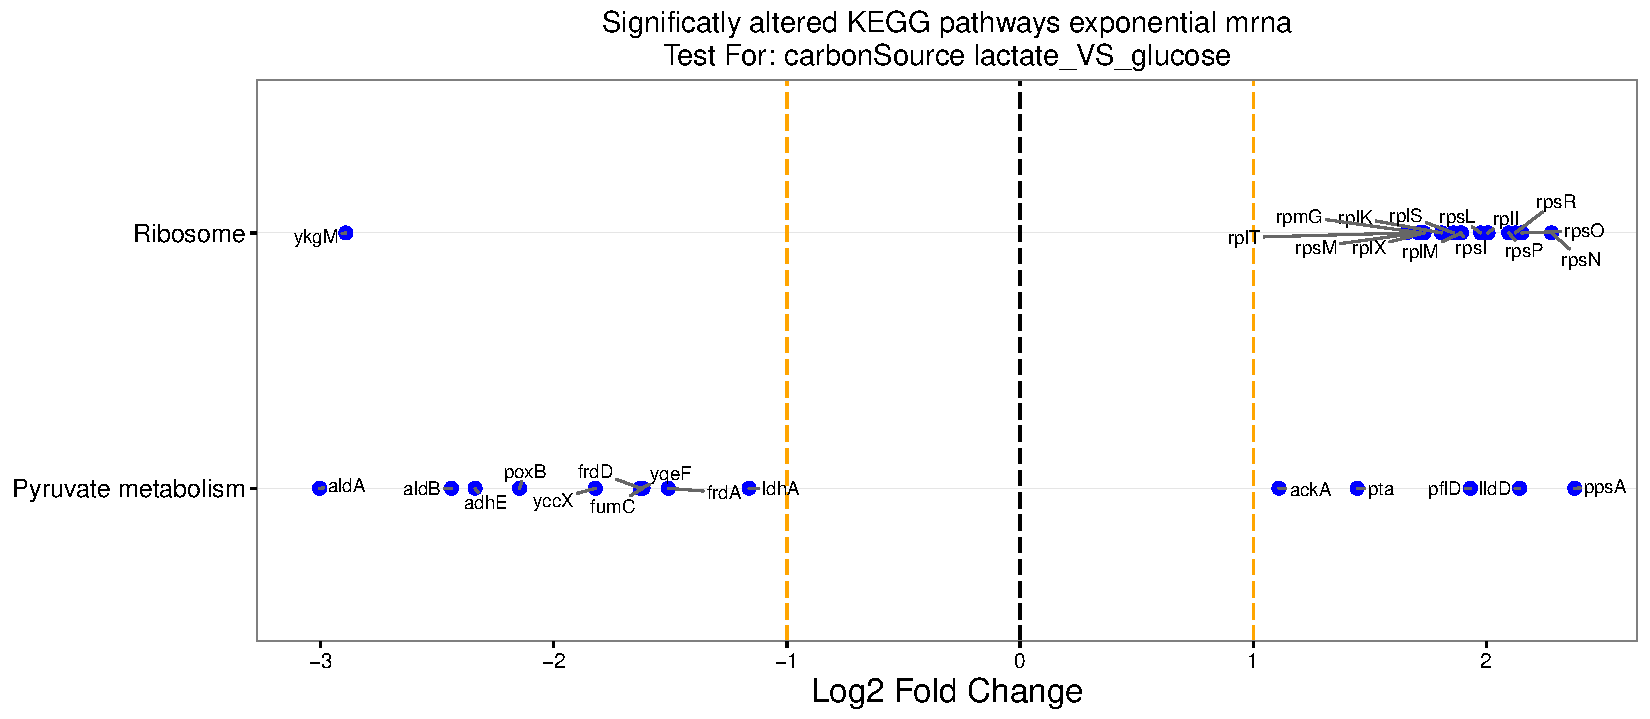
\includegraphics[width=1.0\textwidth]{../../d_figures/kegg_03.pdf}
	\caption[Significantly differentially expressed KEGG pathways for mRNA samples in exponential phase tested for lactate against glucose]
	{\textbf{Significantly differentially expressed KEGG pathways and associated genes with lactate as carbon source, as determined by mRNA abundances in exponential phase.} The top differentially expressed KEGG pathways are shown along the $y$ axis, and the relative fold change of the corresponding genes is shown along the $x$ axis. We show up to 10 of the most significantly changed pathways and for each pathway we show up to 15 of the most significantly changing genes.}
\end{figure}

\clearpage
\begin{figure}
	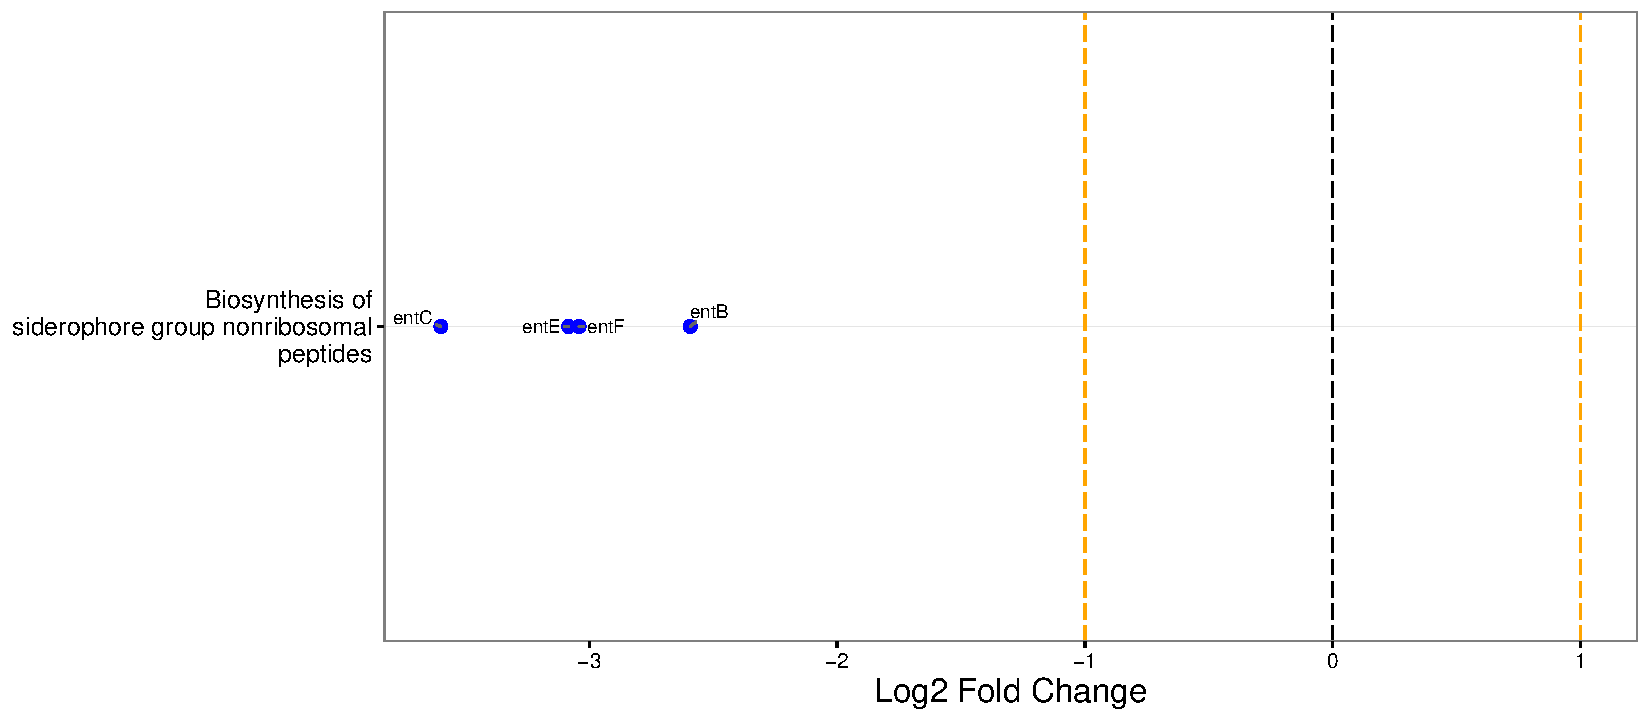
\includegraphics[width=1.0\textwidth]{../../d_figures/kegg_04.pdf}
	\caption[Significantly differentially expressed KEGG pathways for protein samples in exponential phase tested for gluconate against glucose]
	{\textbf{Significantly differentially expressed KEGG pathways and associated genes with gluconate as carbon source, as determined by protein abundances in exponential phase.} The top differentially expressed KEGG pathways are shown along the $y$ axis, and the relative fold change of the corresponding genes is shown along the $x$ axis. We show up to 10 of the most significantly changed pathways and for each pathway we show up to 15 of the most significantly changing genes.}
\end{figure}

\clearpage
\begin{figure}
	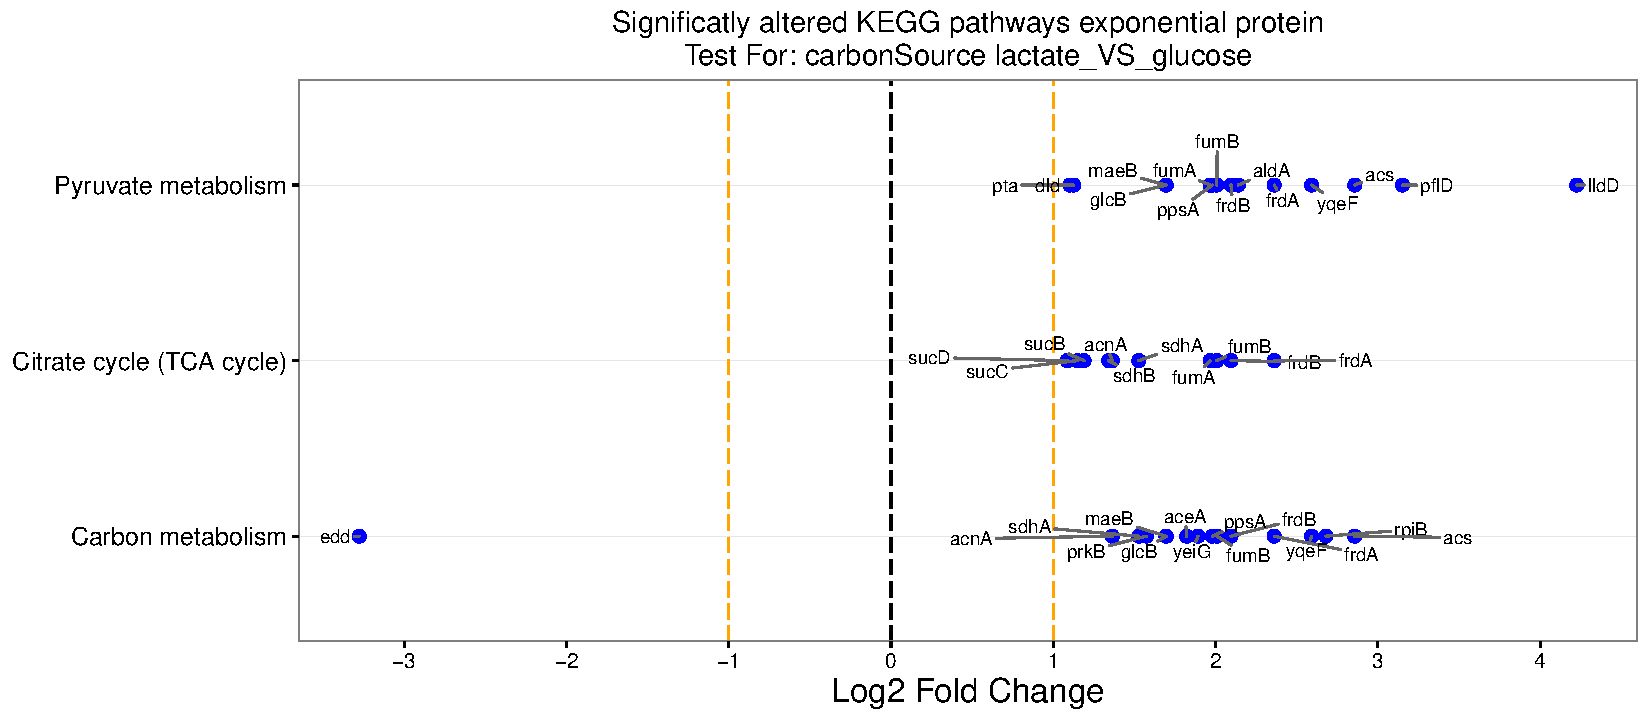
\includegraphics[width=1.0\textwidth]{../../d_figures/kegg_05.pdf}
	\caption[Significantly differentially expressed KEGG pathways for protein samples in exponential phase tested for lactate against glucose]
	{\textbf{Significantly differentially expressed KEGG pathways and associated genes with lactate as carbon source, as determined by protein abundances in exponential phase.} The top differentially expressed KEGG pathways are shown along the $y$ axis, and the relative fold change of the corresponding genes is shown along the $x$ axis. We show up to 10 of the most significantly changed pathways and for each pathway we show up to 15 of the most significantly changing genes.}
\end{figure}

\clearpage
\begin{figure}
	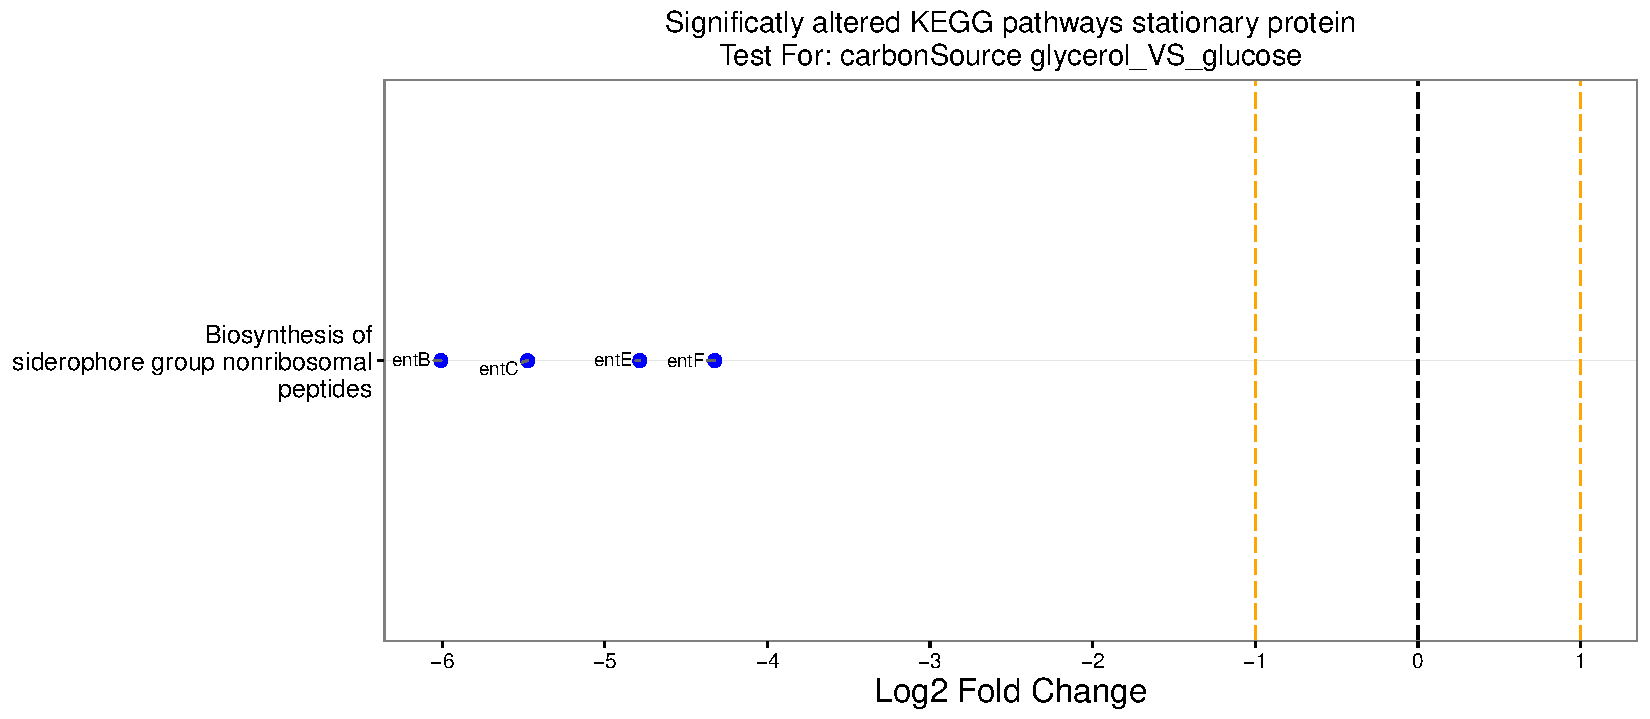
\includegraphics[width=1.0\textwidth]{../../d_figures/kegg_06.pdf}
	\caption[Significantly differentially expressed KEGG pathways for protein samples in stationary phase tested for glycerol against glucose]
	{\textbf{Significantly differentially expressed KEGG pathways and associated genes with glycerol as carbon source, as determined by protein abundances in stationary phase.} The top differentially expressed KEGG pathways are shown along the $y$ axis, and the relative fold change of the corresponding genes is shown along the $x$ axis. We show up to 10 of the most significantly changed pathways and for each pathway, we show up to 15 of the most significantly changing genes.}
\end{figure}

\clearpage
\begin{figure}
	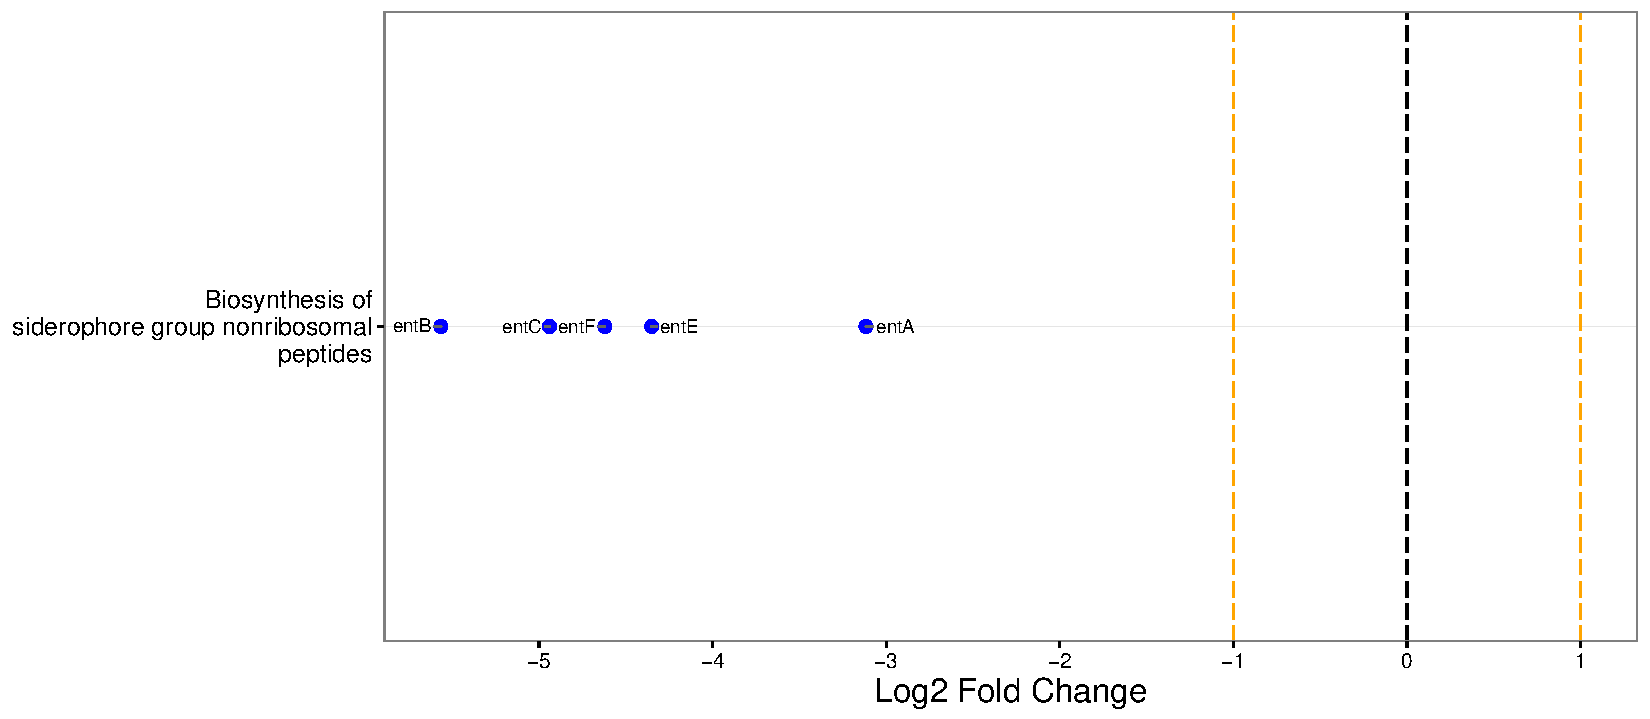
\includegraphics[width=1.0\textwidth]{../../d_figures/kegg_07.pdf}
	\caption[Significantly differentially expressed KEGG pathways for protein samples in stationary phase tested for gluconate against glucose]
	{\textbf{Significantly differentially expressed KEGG pathways and associated genes with gluconate as carbon source, as determined by protein abundances in stationary phase.} The top differentially expressed KEGG pathways are shown along the $y$ axis, and the relative fold change of the corresponding genes is shown along the $x$ axis. We show up to 10 of the most significantly changed pathways and for each pathway, we show up to 15 of the most significantly changing genes.}
\end{figure}

\clearpage
\begin{figure}
	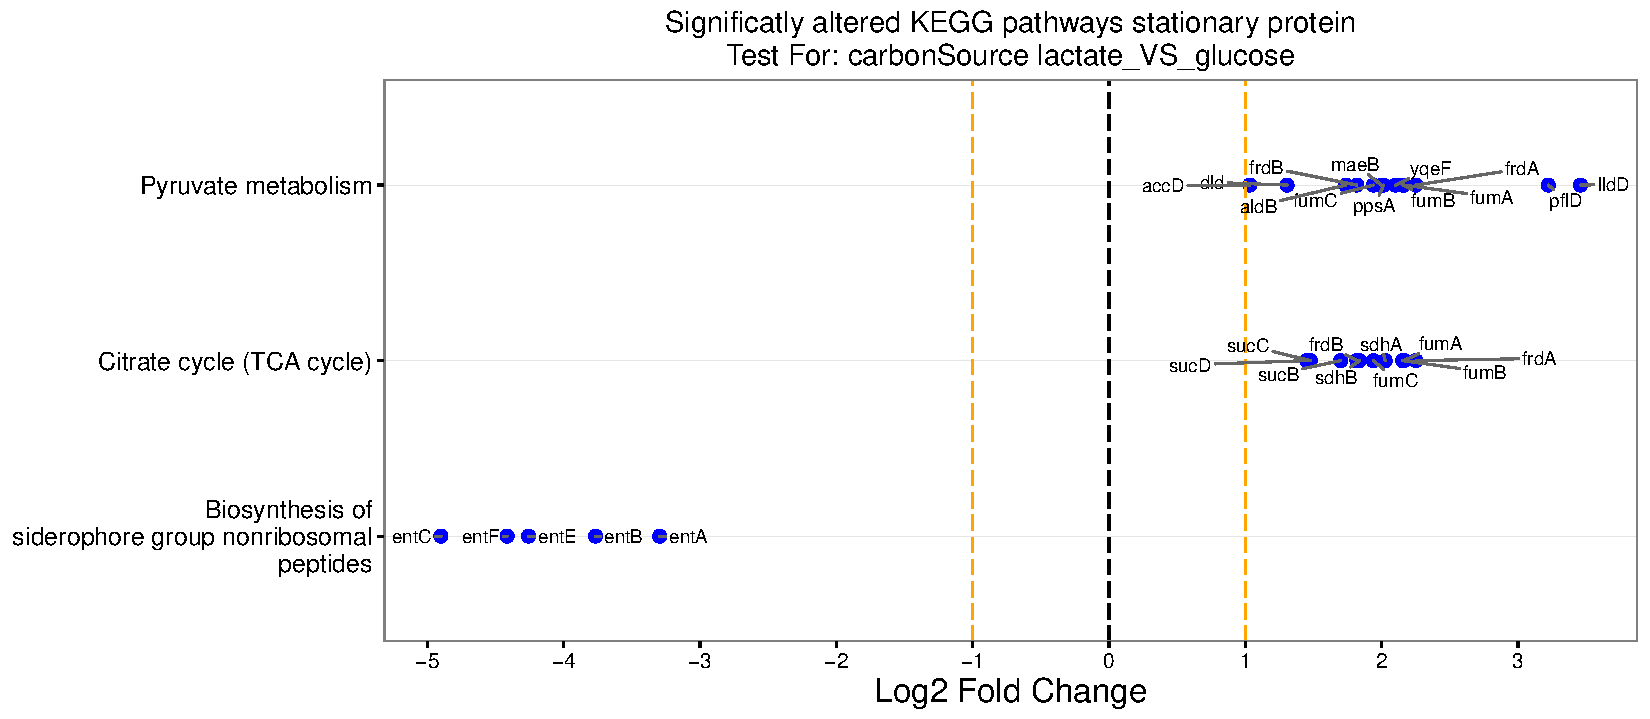
\includegraphics[width=1.0\textwidth]{../../d_figures/kegg_08.pdf}
	\caption[Significantly differentially expressed KEGG pathways for protein samples in stationary phase tested for lactate against glucose]
	{\textbf{Significantly differentially expressed KEGG pathways and associated genes with lactate as carbon source, as determined by protein abundances in stationary phase.} The top differentially expressed KEGG pathways are shown along the $y$ axis, and the relative fold change of the corresponding genes is shown along the $x$ axis. We show up to 10 of the most significantly changed pathways and for each pathway, we show up to 15 of the most significantly changing genes.}
\end{figure}

\clearpage
\begin{figure}
	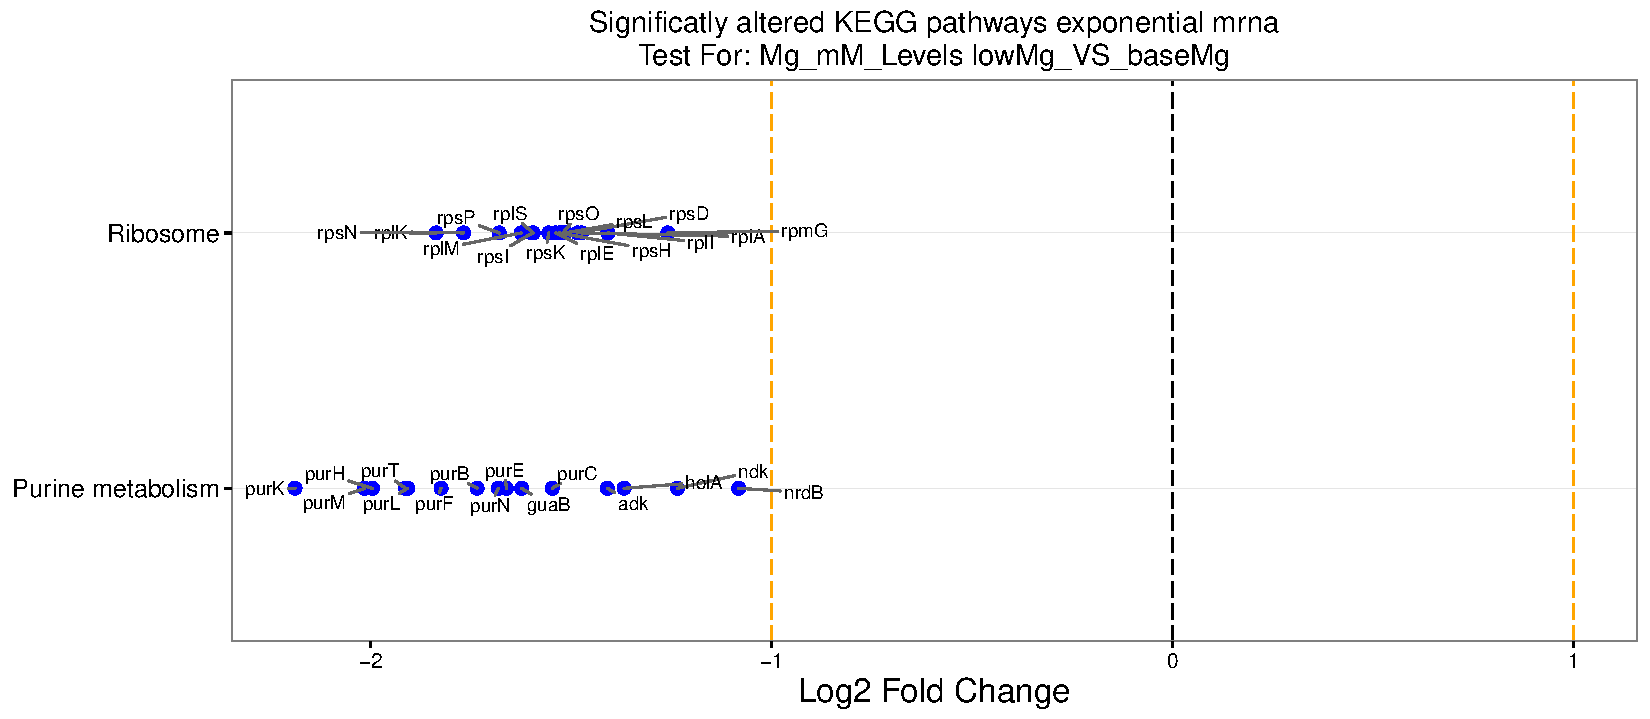
\includegraphics[width=1.0\textwidth]{../../d_figures/kegg_09.pdf}
	\caption[Significantly differentially expressed KEGG pathways for mRNA samples in exponential phase tested for low Mg\textsuperscript{2+} levels against base Mg\textsuperscript{2+}]
	{\textbf{Significantly differentially expressed KEGG pathways and associated genes with low Mg\textsuperscript{2+} levels, as determined by mRNA abundances in exponential phase.} The top differentially expressed KEGG pathways are shown along the $y$ axis, and the relative fold change of the corresponding genes is shown along the $x$ axis. We show up to 10 of the most significantly changed pathways and for each pathway, we show up to 15 of the most significantly changing genes.}
\end{figure}

\clearpage
\begin{figure}
	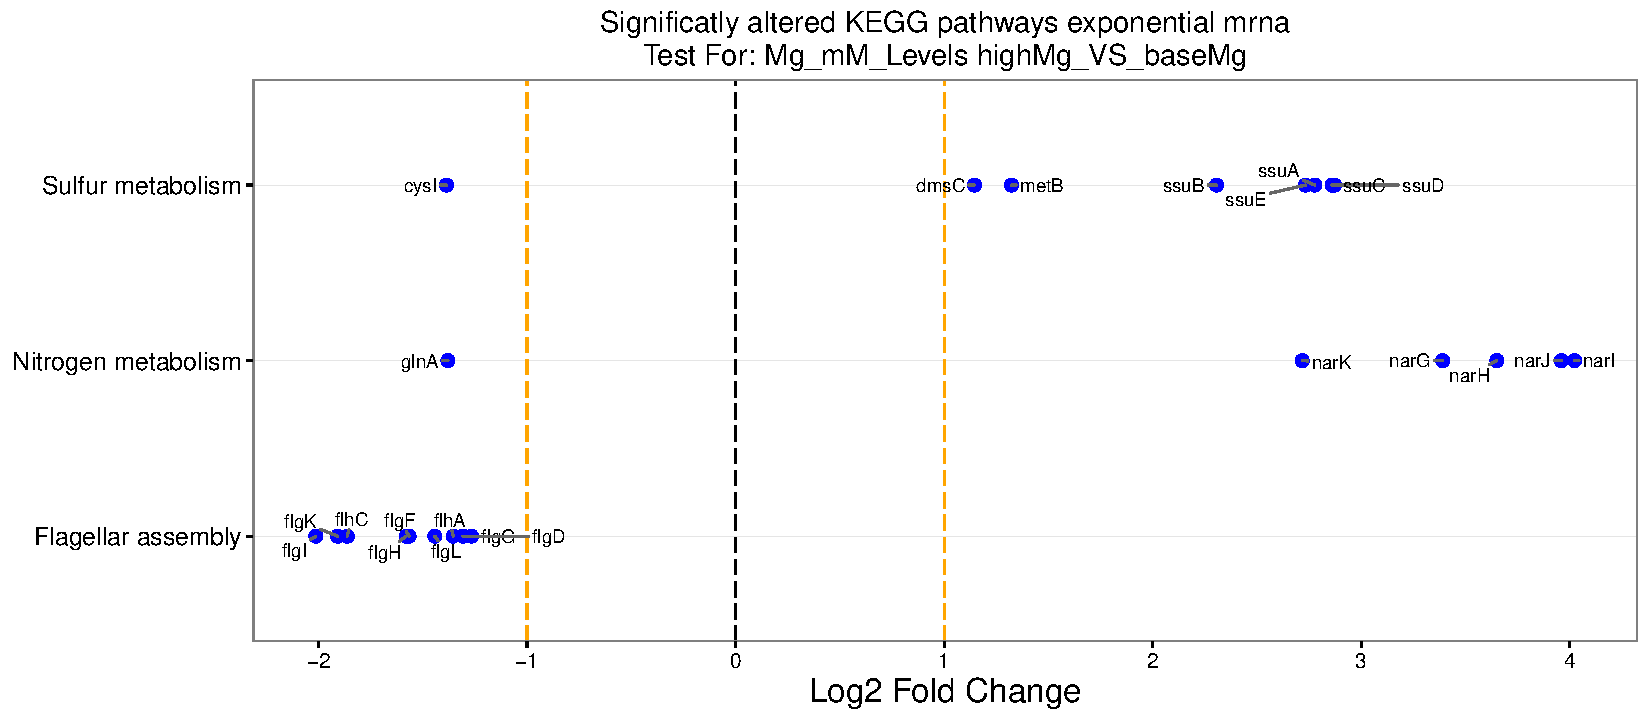
\includegraphics[width=1.0\textwidth]{../../d_figures/kegg_10.pdf}
	\caption[Significantly differentially expressed KEGG pathways for mRNA samples in exponential phase tested for high Mg\textsuperscript{2+} against base Mg\textsuperscript{2+}]
	{\textbf{Significantly differentially expressed KEGG pathways and associated genes with high Mg\textsuperscript{2+} levels, as determined by mRNA abundances in exponential phase.} The top differentially expressed KEGG pathways are shown along the $y$ axis, and the relative fold change of the corresponding genes is shown along the $x$ axis. We show up to 10 of the most significantly changed pathways and for each pathway, we show up to 15 of the most significantly changing genes.}
\end{figure}

\clearpage
\begin{figure}
	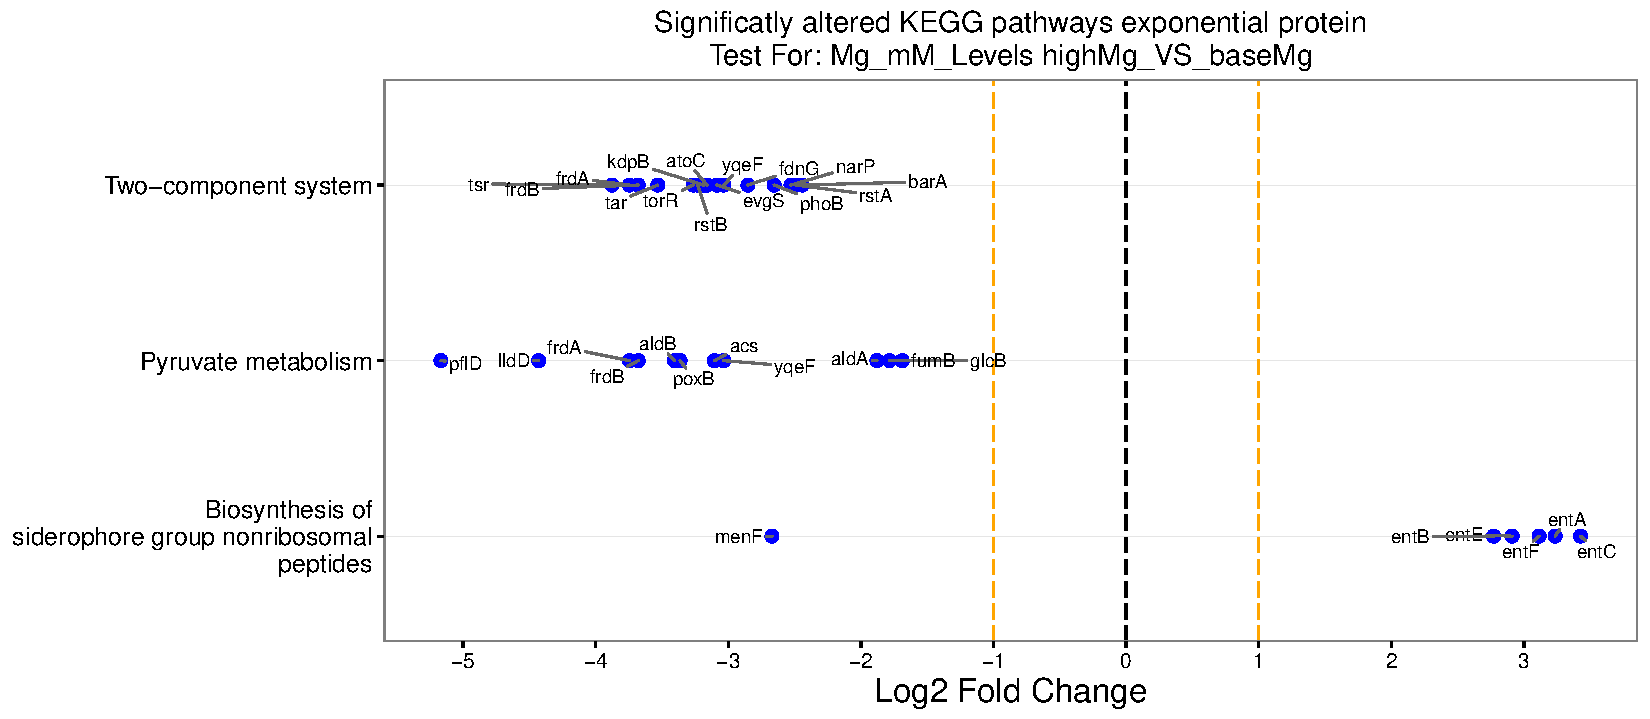
\includegraphics[width=1.0\textwidth]{../../d_figures/kegg_11.pdf}
	\caption[Significantly differentially expressed KEGG pathways for protein samples in exponential phase tested for high Mg\textsuperscript{2+} against base Mg\textsuperscript{2+}]
	{\textbf{Significantly differentially expressed KEGG pathways and associated genes with high Mg\textsuperscript{2+} levels, as determined by protein abundances in exponential phase.} The top differentially expressed KEGG pathways are shown along the $y$ axis, and the relative fold change of the corresponding genes is shown along the $x$ axis. We show up to 10 of the most significantly changed pathways and for each pathway, we show up to 15 of the most significantly changing genes.}
\end{figure}

\clearpage
\begin{figure}
	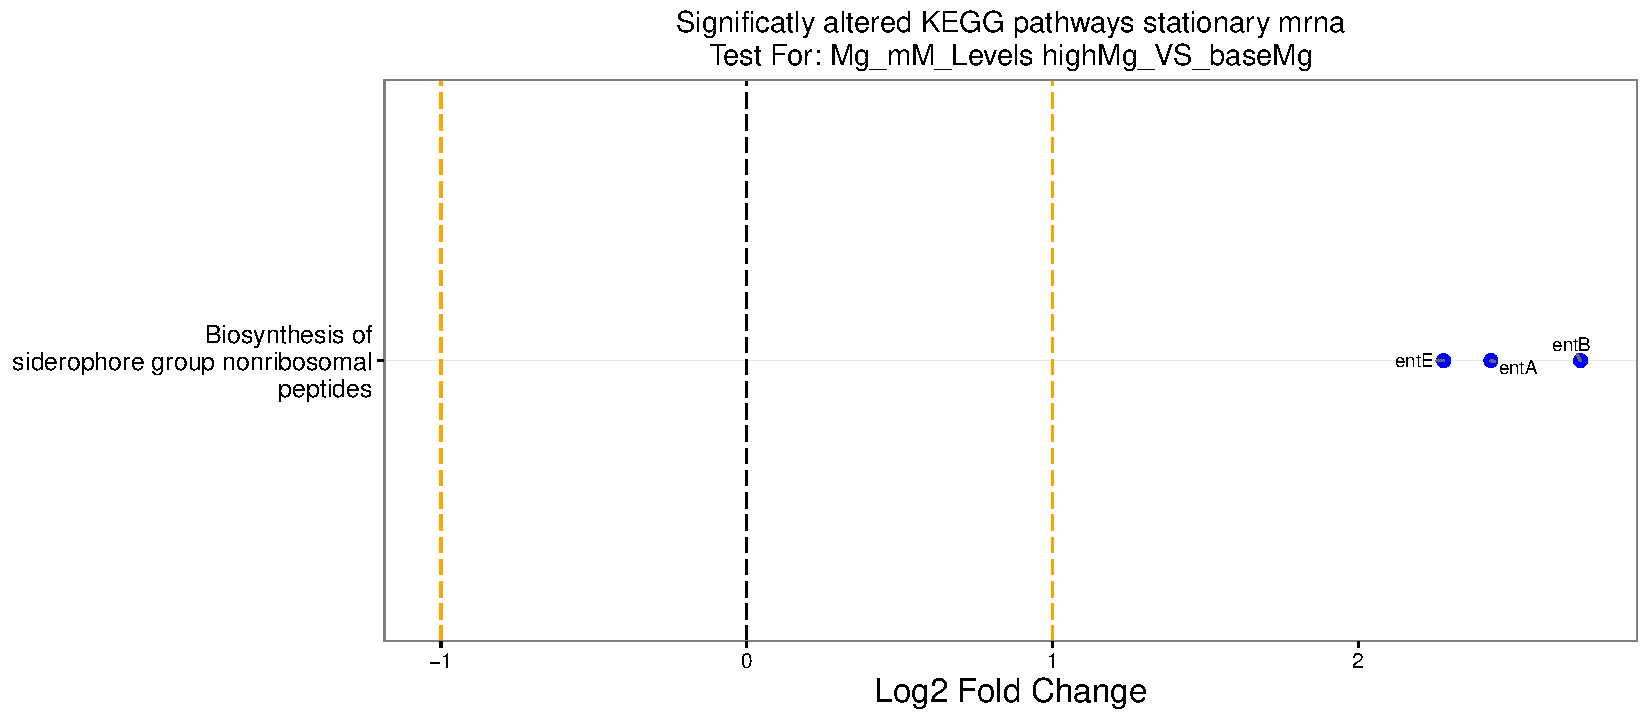
\includegraphics[width=1.0\textwidth]{../../d_figures/kegg_12.pdf}
	\caption[Significantly differentially expressed KEGG pathways for mRNA samples in stationary phase tested for high Mg\textsuperscript{2+} against base Mg\textsuperscript{2+}]
	{\textbf{Significantly differentially expressed KEGG pathways and associated genes with high Mg\textsuperscript{2+} levels, as determined by mRNA abundances in stationary phase.} The top differentially expressed KEGG pathways are shown along the $y$ axis, and the relative fold change of the corresponding genes is shown along the $x$ axis. We show up to 10 of the most significantly changed pathways and for each pathway, we show up to 15 of the most significantly changing genes.}
\end{figure}

\clearpage
\begin{figure}
	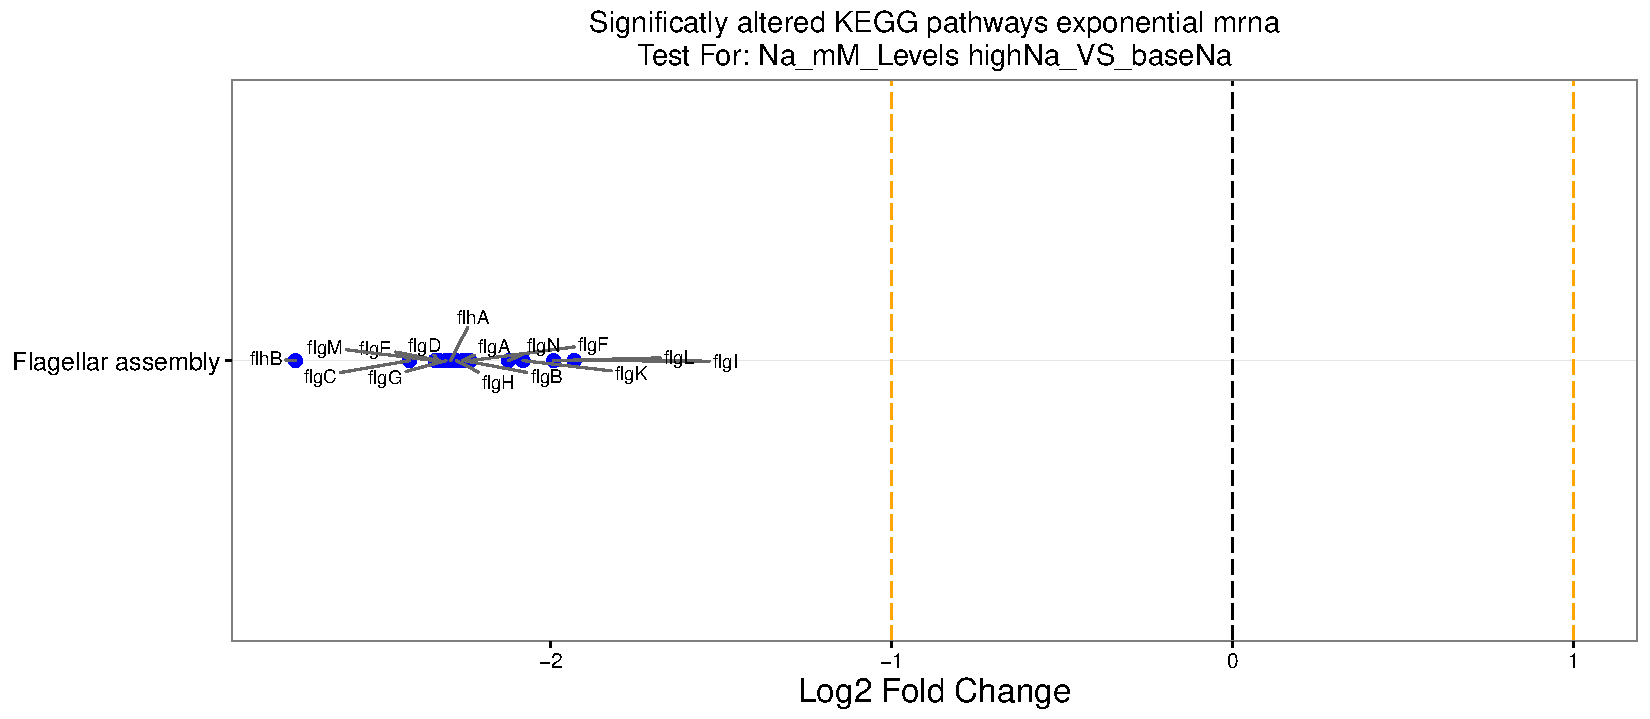
\includegraphics[width=1.0\textwidth]{../../d_figures/kegg_13.pdf}
	\caption[Significantly differentially expressed KEGG pathways for mRNA samples in exponential phase tested for high Na\textsuperscript{+} against base Na\textsuperscript{+}]
	{\textbf{Significantly differentially expressed KEGG pathways and associated genes with high Na\textsuperscript{+} levels, as determined by mRNA abundances in exponential phase.} The top differentially expressed KEGG pathways are shown along the $y$ axis, and the relative fold change of the corresponding genes is shown along the $x$ axis. We show up to 10 of the most significantly changed pathways and for each pathway, we show up to 15 of the most significantly changing genes.}
\end{figure}

\clearpage
\begin{figure}
	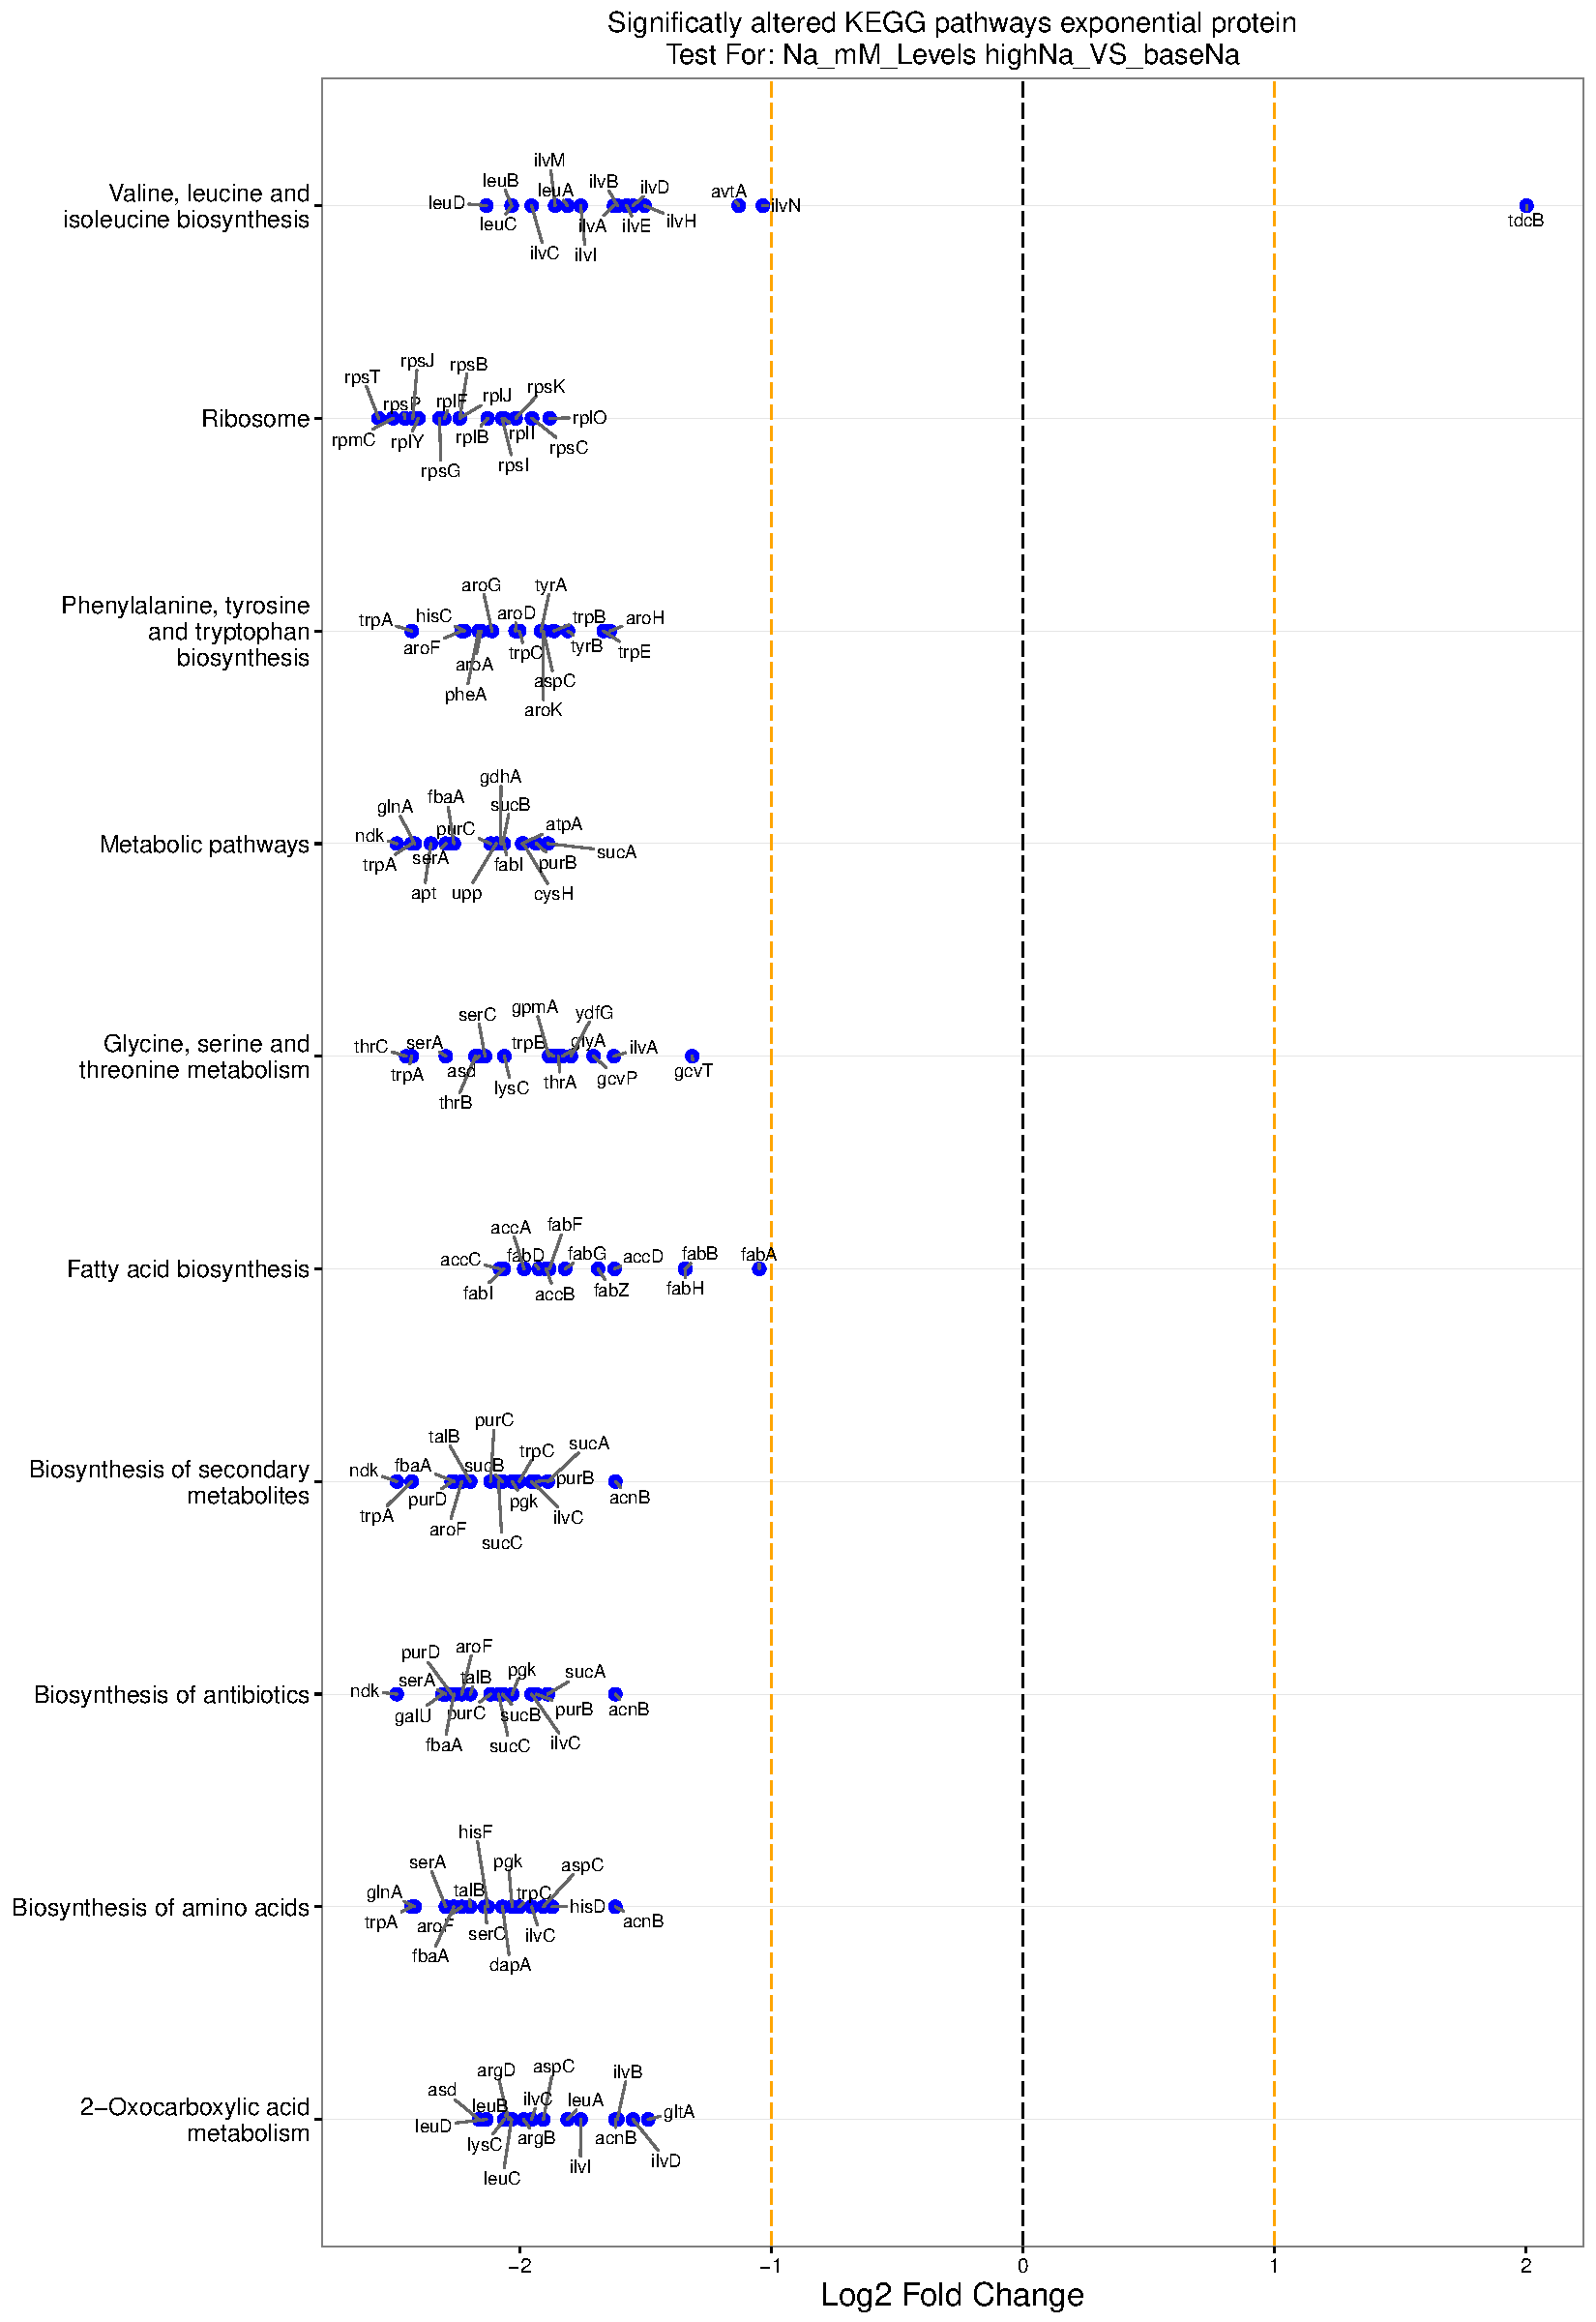
\includegraphics[width=1.0\textwidth]{../../d_figures/kegg_14.pdf}
	\caption[Significantly differentially expressed KEGG pathways for protein samples in exponential phase tested for high Na\textsuperscript{+} against base Na\textsuperscript{+}]
	{\textbf{Significantly differentially expressed KEGG pathways and associated genes with high Na\textsuperscript{+} levels, as determined by protein abundances in exponential phase.} The top differentially expressed KEGG pathways are shown along the $y$ axis, and the relative fold change of the corresponding genes is shown along the $x$ axis. We show up to 10 of the most significantly changed pathways and for each pathway, we show up to 15 of the most significantly changing genes.}
\end{figure}

\clearpage
\begin{figure}
	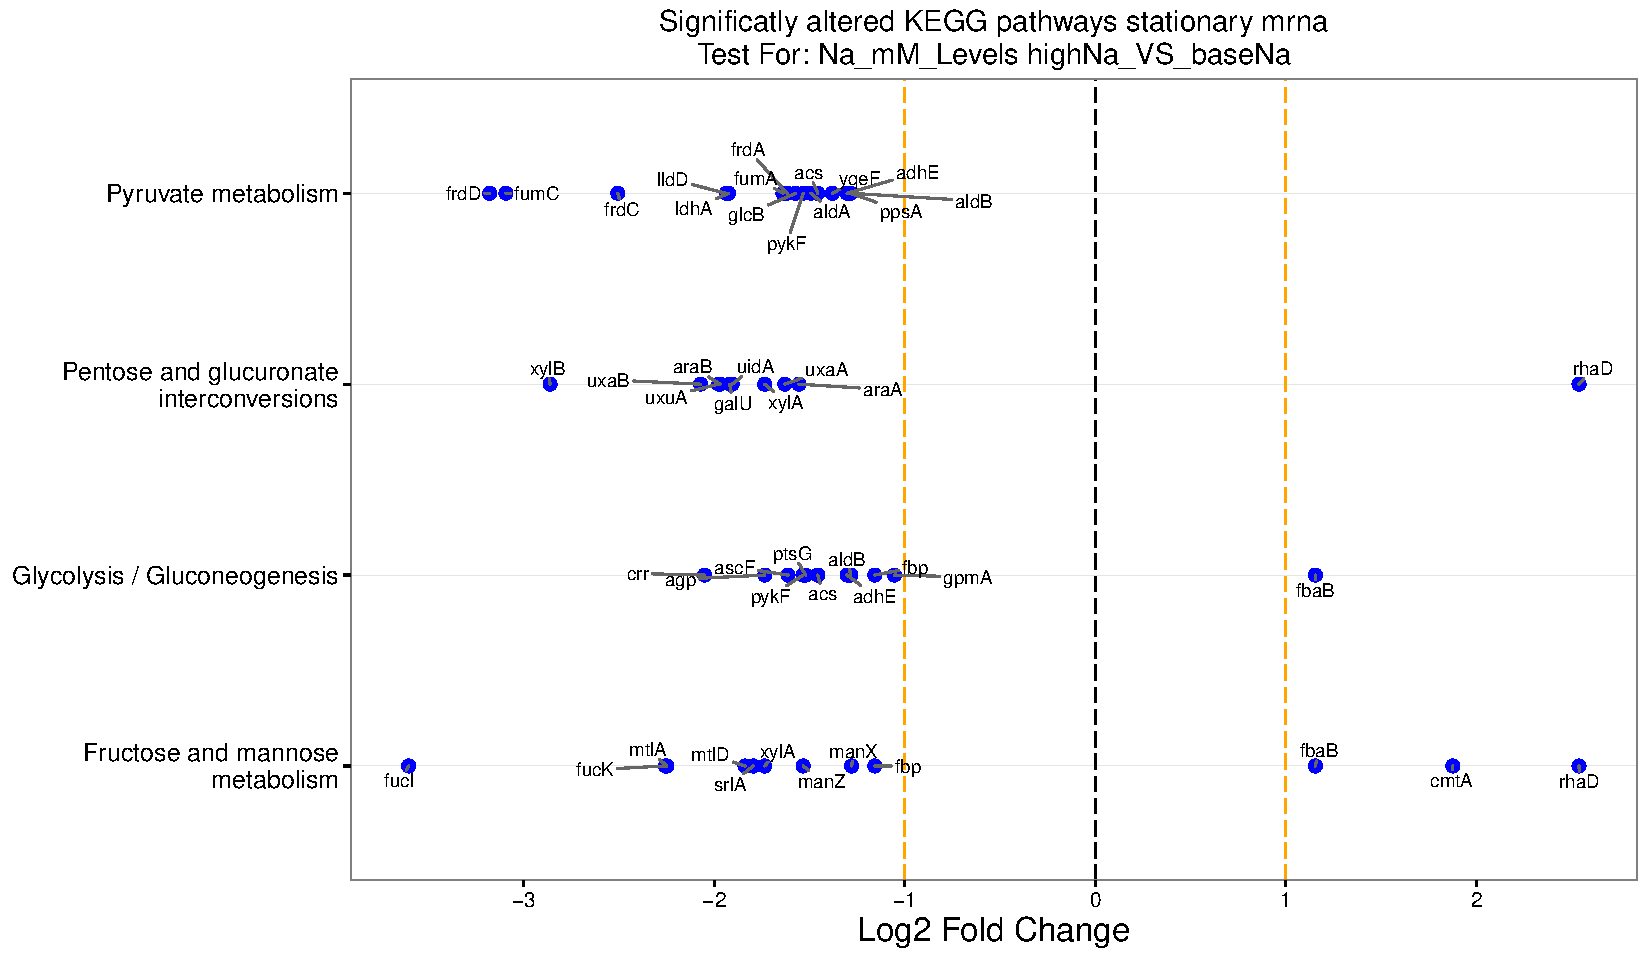
\includegraphics[width=1.0\textwidth]{../../d_figures/kegg_15.pdf}
	\caption[Significantly differentially expressed KEGG pathways for mRNA samples in stationary phase tested for high Na\textsuperscript{+} against base Na\textsuperscript{+}]
	{\textbf{Significantly differentially expressed KEGG pathways and associated genes with high Na\textsuperscript{+} levels, as determined by mRNA abundances in stationary phase.} The top differentially expressed KEGG pathways are shown along the $y$ axis, and the relative fold change of the corresponding genes is shown along the $x$ axis. We show up to 10 of the most significantly changed pathways and for each pathway, we show up to 15 of the most significantly changing genes.}
\end{figure}

\clearpage
\begin{figure}
	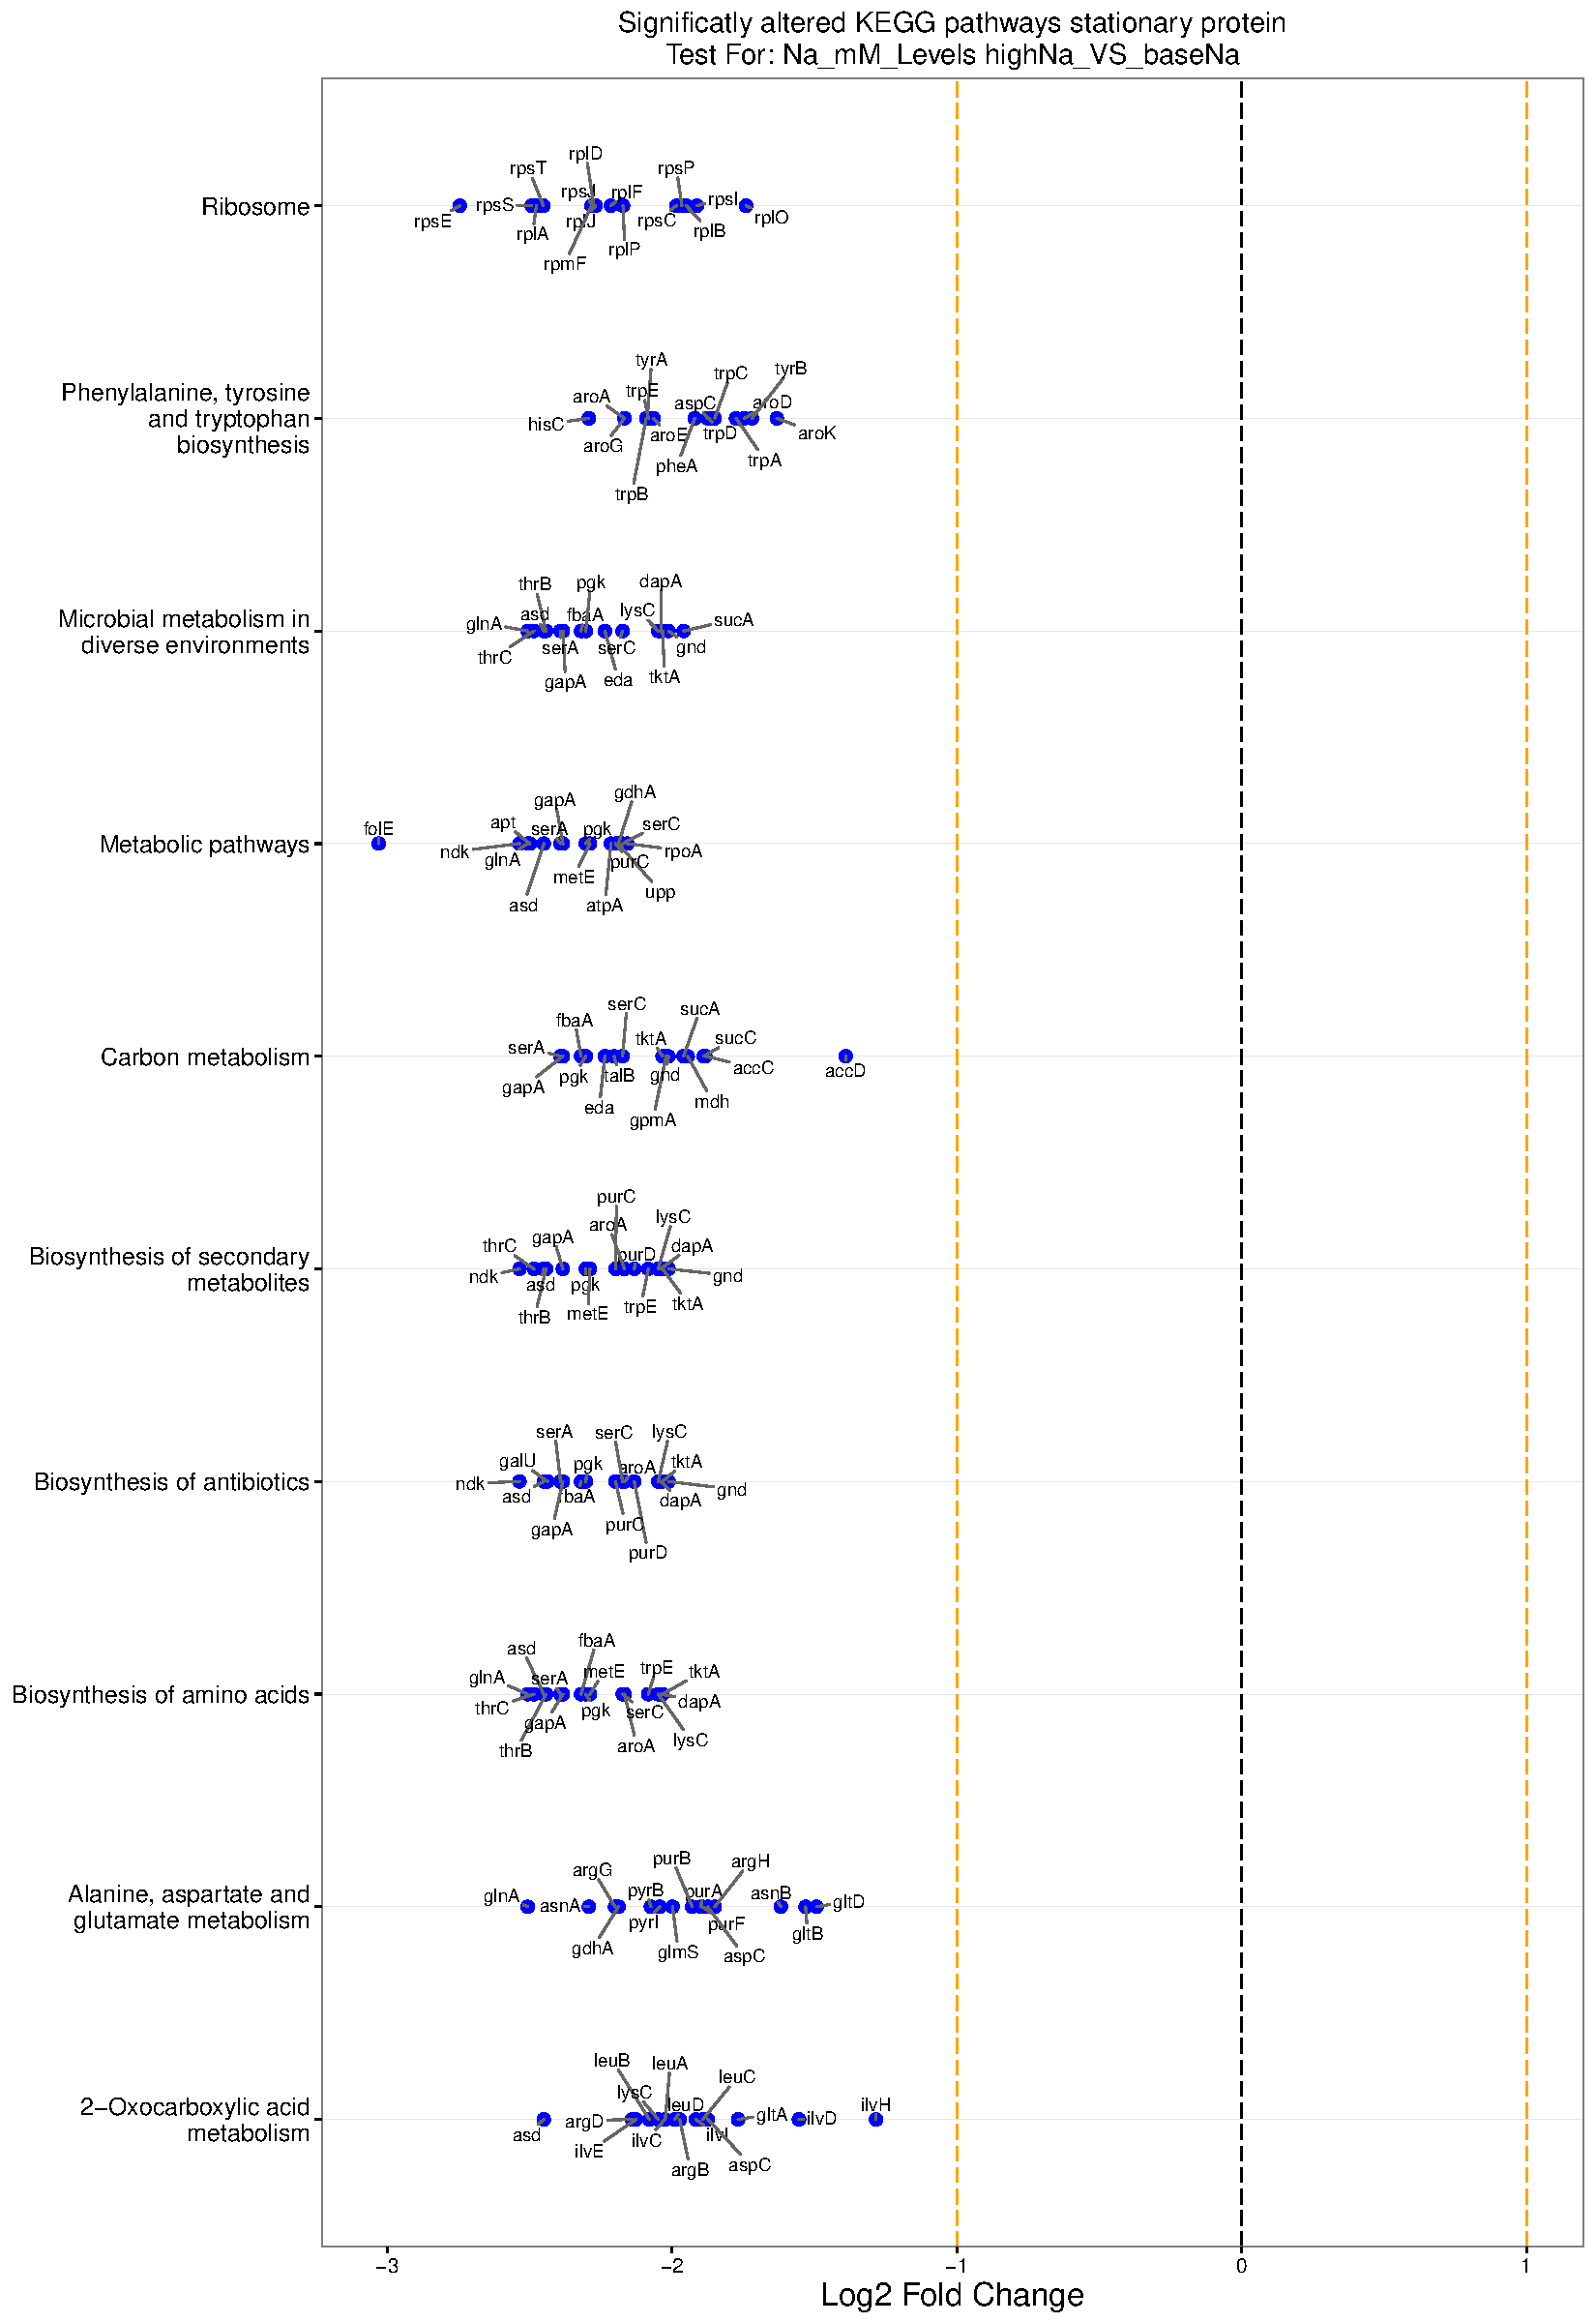
\includegraphics[width=1.0\textwidth]{../../d_figures/kegg_16.pdf}
	\caption[Significantly differentially expressed KEGG pathways for protein samples in stationary phase tested for high Na\textsuperscript{+} against base Na\textsuperscript{+}]
	{\textbf{Significantly differentially expressed KEGG pathways and associated genes with high Na\textsuperscript{+} levels, as determined by protein abundances in stationary phase.} The top differentially expressed KEGG pathways are shown along the $y$ axis, and the relative fold change of the corresponding genes is shown along the $x$ axis. We show up to 10 of the most significantly changed pathways and for each pathway, we show up to 15 of the most significantly changing genes.}
\end{figure}
\clearpage


\begin{figure}[!htb]
	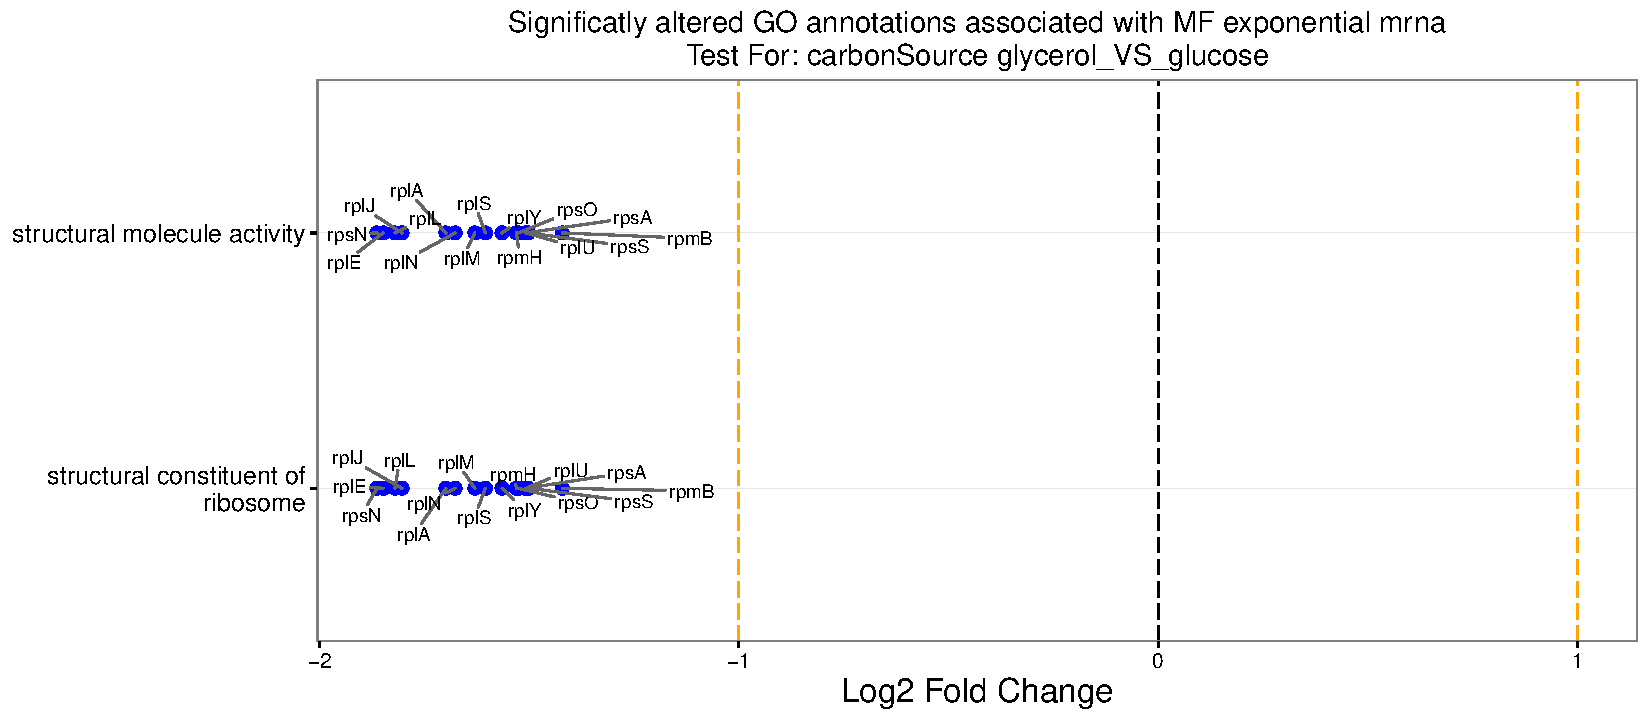
\includegraphics[width=1.0\textwidth]{../../d_figures/mf_n_01.pdf}
	\caption[Significantly differentially expressed GO annotations associated with molecular functions for mRNA samples in exponential phase tested for glycerol against glucose]
	{\textbf{Significantly differentially expressed GO annotations related with molecular functions and associated genes with glycerol as carbon source, as determined by mRNA abundances in exponential phase.} The top differentially expressed KEGG pathways are shown along the $y$ axis, and the relative fold change of the corresponding genes is shown along the $x$ axis. We show up to 10 of the most significantly changed pathways and for each pathway, we show up to 15 of the most significantly changing genes.}
\end{figure}

\clearpage
\begin{figure}
	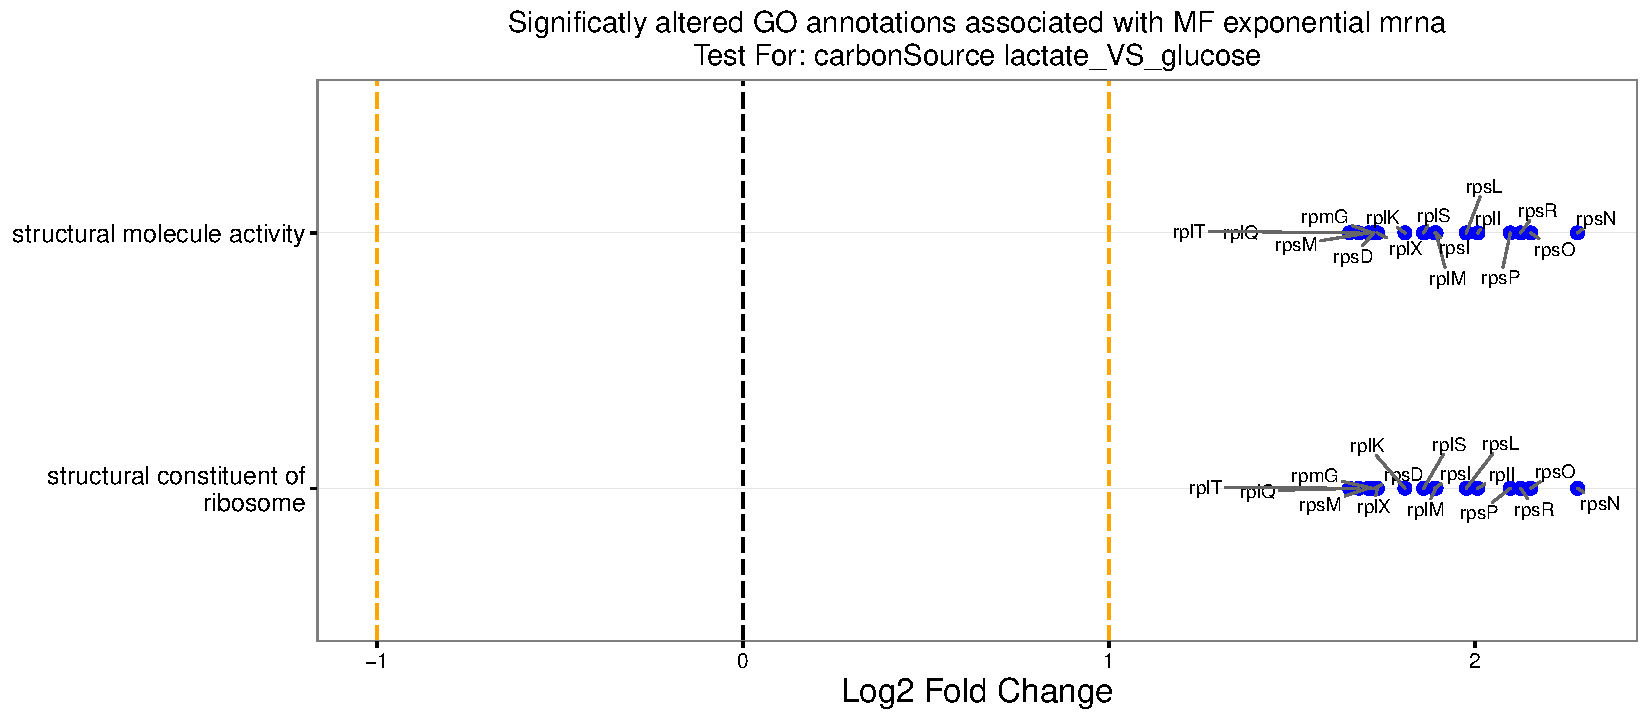
\includegraphics[width=1.0\textwidth]{../../d_figures/mf_n_02.pdf}
	\caption[Significantly differentially expressed GO annotations associated with molecular functions for mRNA samples in exponential phase tested for lactate against glucose]
	{\textbf{Significantly differentially expressed GO annotations related with molecular functions and associated genes with lactate as carbon source, as determined by mRNA abundances in exponential phase.} The top differentially expressed KEGG pathways are shown along the $y$ axis, and the relative fold change of the corresponding genes is shown along the $x$ axis. We show up to 10 of the most significantly changed pathways and for each pathway, we show up to 15 of the most significantly changing genes.}
\end{figure}

\clearpage
\begin{figure}
	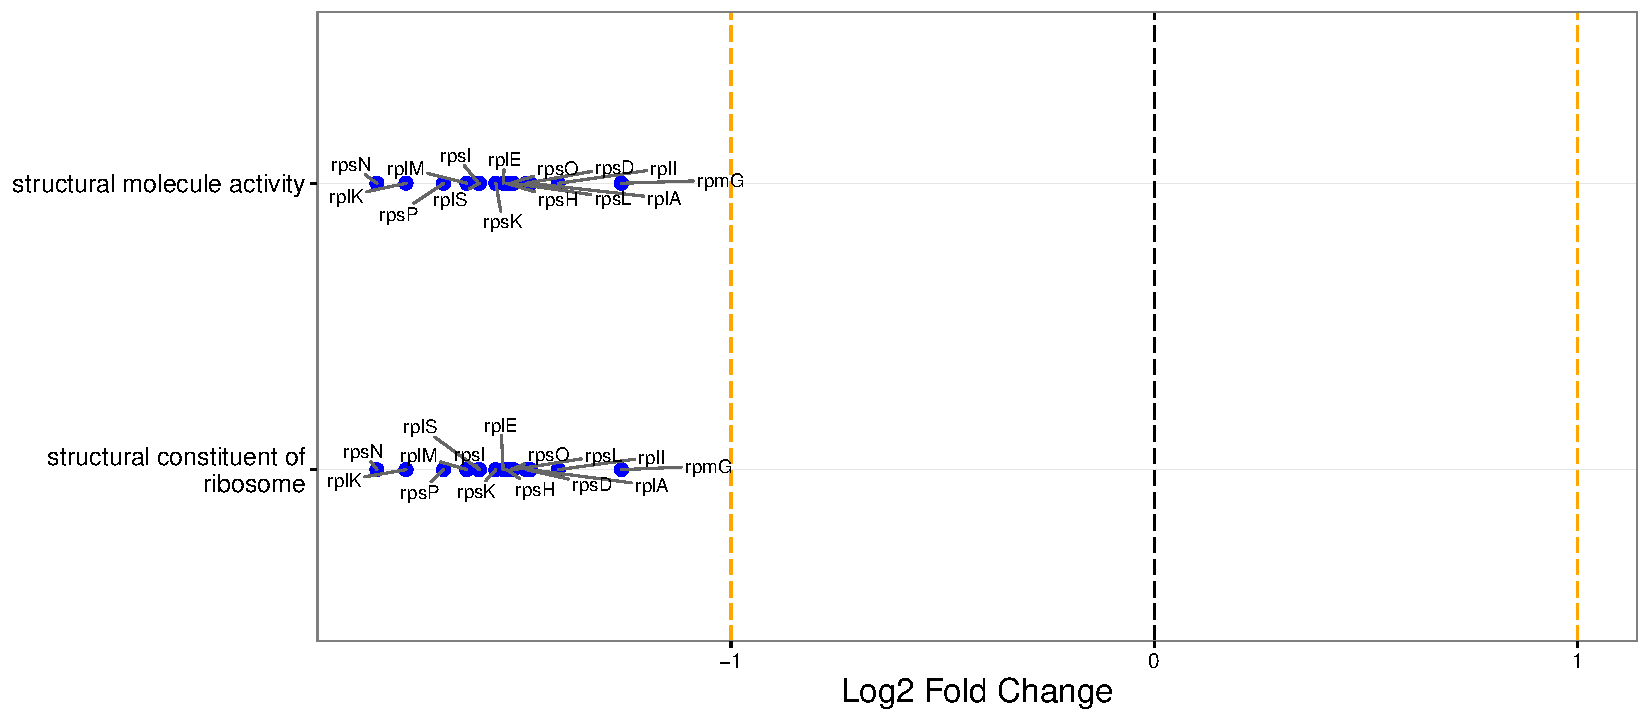
\includegraphics[width=1.0\textwidth]{../../d_figures/mf_n_03.pdf}
	\caption[Significantly differentially expressed GO annotations associated with molecular functions for mRNA samples in exponential phase tested for low Mg\textsuperscript{2+} against base Mg\textsuperscript{2+}]
	{\textbf{Significantly differentially expressed GO annotations related with molecular functions and associated genes with low Mg\textsuperscript{2+} levels, as determined by mRNA abundances in exponential phase.} The top differentially expressed KEGG pathways are shown along the $y$ axis, and the relative fold change of the corresponding genes is shown along the $x$ axis. We show up to 10 of the most significantly changed pathways and for each pathway, we show up to 15 of the most significantly changing genes.}
\end{figure}

\clearpage
\begin{figure}
	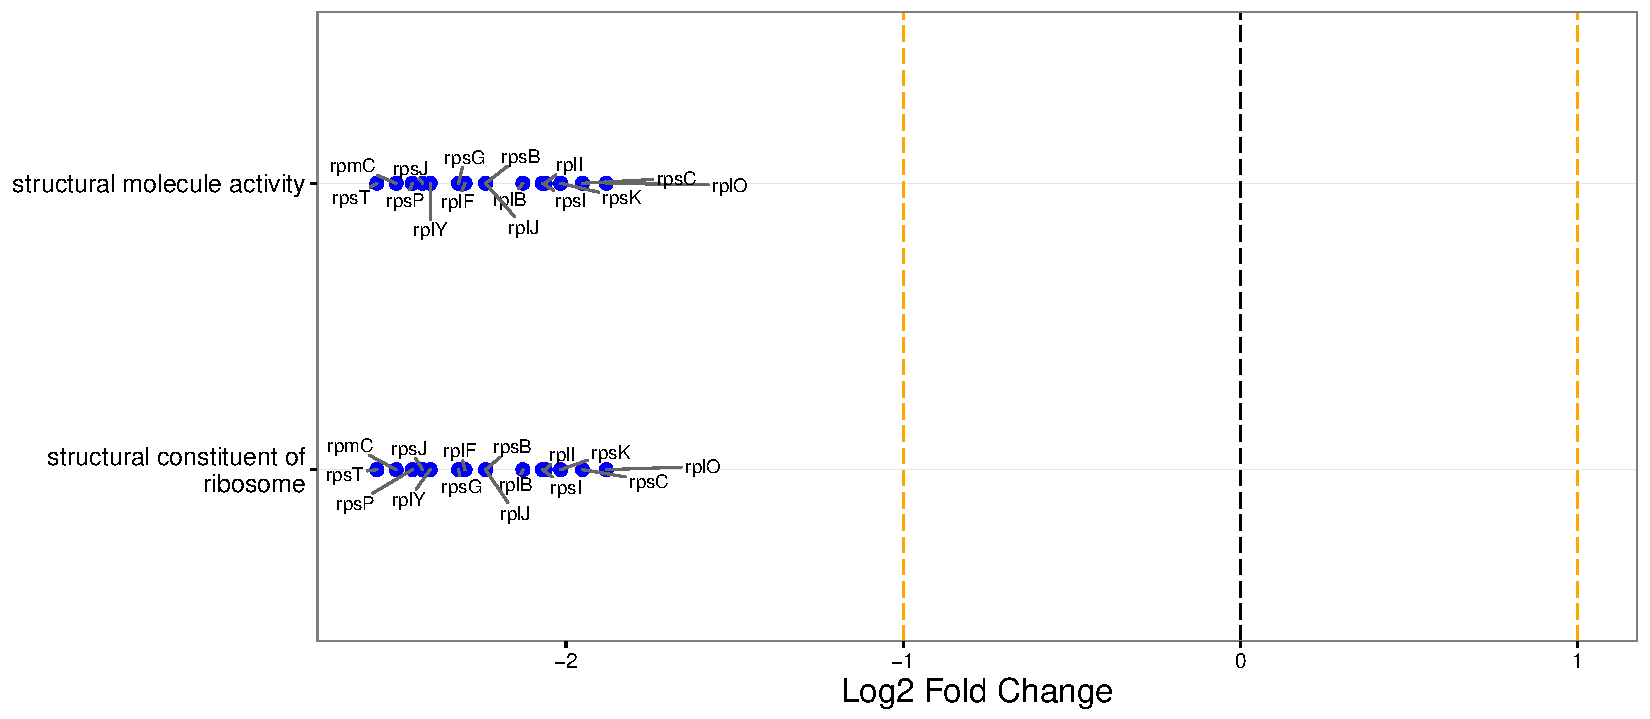
\includegraphics[width=1.0\textwidth]{../../d_figures/mf_n_04.pdf}
	\caption[Significantly differentially expressed GO annotations associated with molecular functions for protein samples in exponential phase tested for high Na\textsuperscript{+} against base Na\textsuperscript{+}]
	{\textbf{Significantly differentially expressed GO annotations related with molecular functions and associated genes with high Na\textsuperscript{+} levels, as determined by protein abundances in exponential phase.} The top differentially expressed KEGG pathways are shown along the $y$ axis, and the relative fold change of the corresponding genes is shown along the $x$ axis. We show up to 10 of the most significantly changed pathways and for each pathway, we show up to 15 of the most significantly changing genes.}
\end{figure}

\clearpage
\begin{figure}
	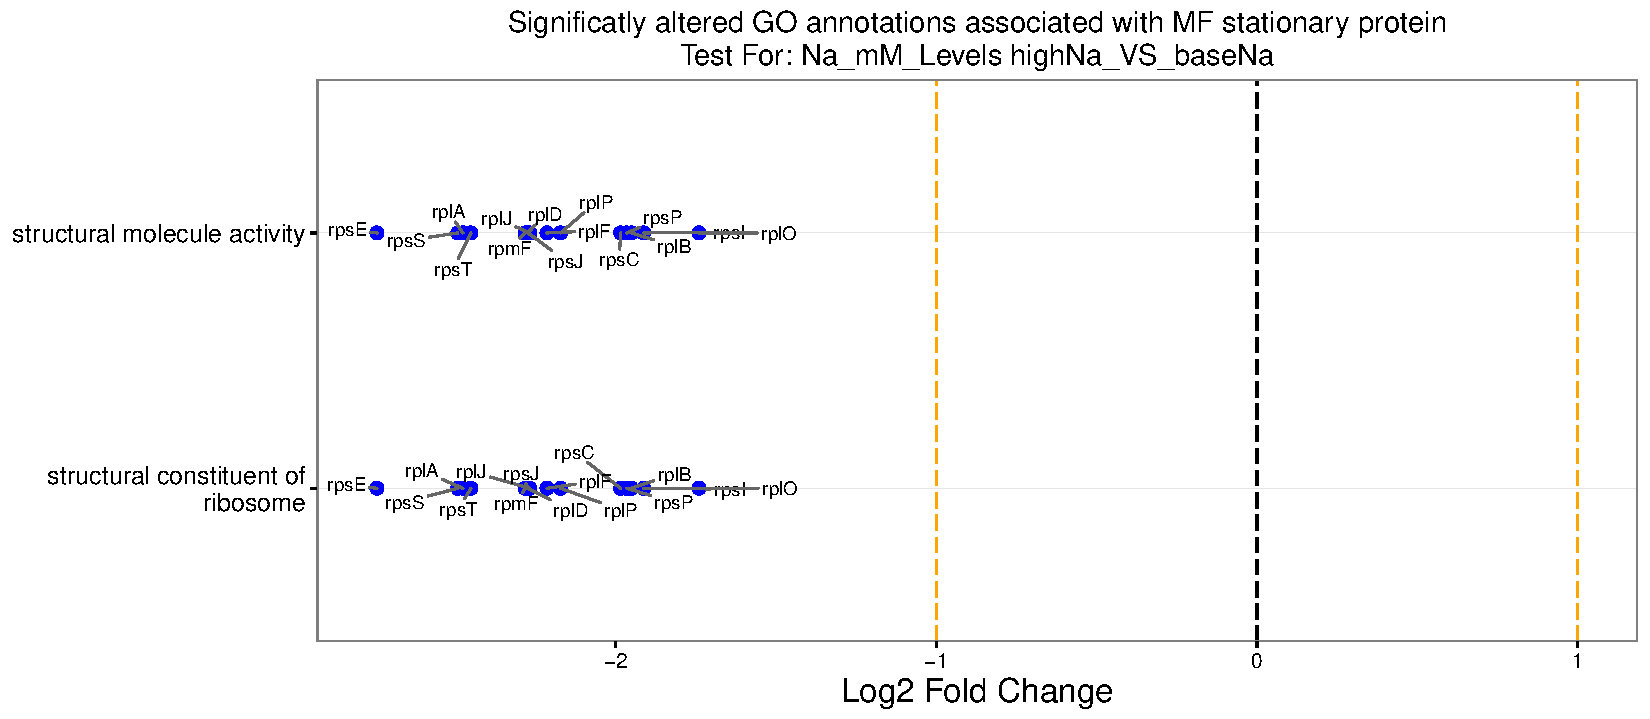
\includegraphics[width=1.0\textwidth]{../../d_figures/mf_n_05.pdf}
	\caption[Significantly differentially expressed GO annotations associated with molecular functions for protein samples in stationary phase tested for high Na\textsuperscript{+} against base Na\textsuperscript{+}]
	{\textbf{Significantly differentially expressed GO annotations related with molecular functions and associated genes with high Na\textsuperscript{+} levels, as determined by protein abundances in stationary phase.} The top differentially expressed KEGG pathways are shown along the $y$ axis, and the relative fold change of the corresponding genes is shown along the $x$ axis. We show up to 10 of the most significantly changed pathways and for each pathway, we show up to 15 of the most significantly changing genes.}
\end{figure}

\clearpage
\begin{figure}[!htb]
	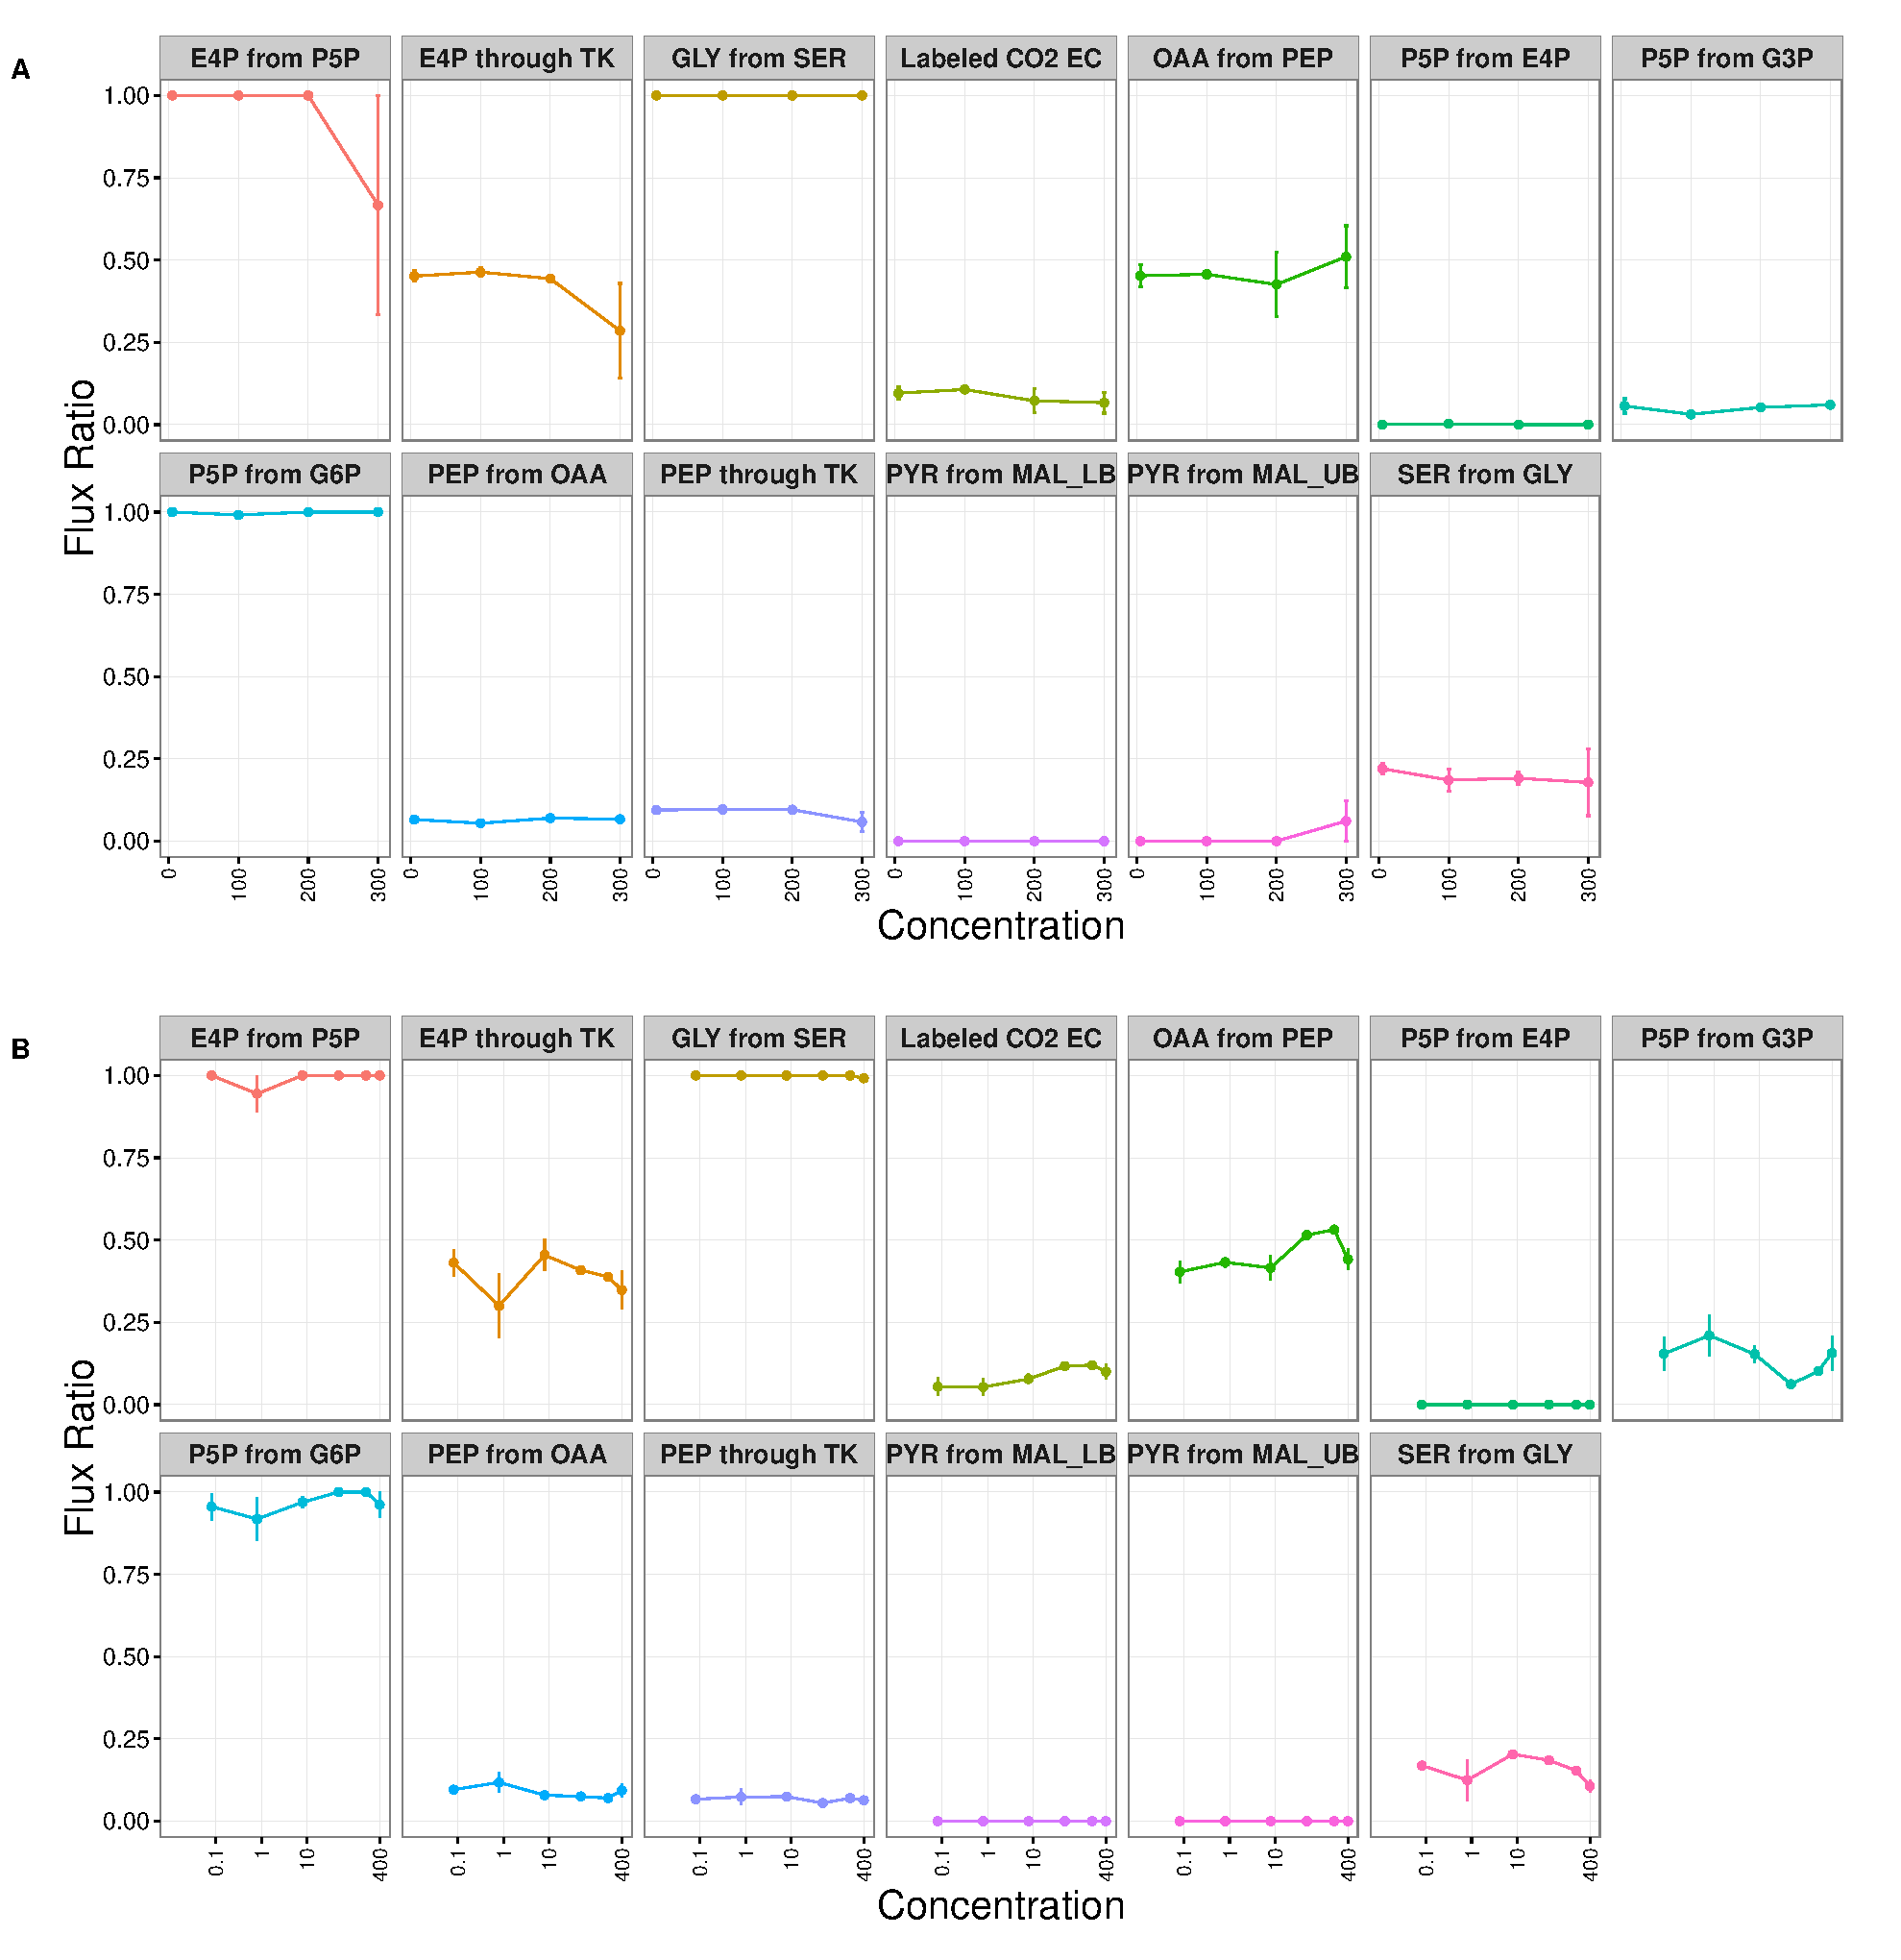
\includegraphics[width=1\textwidth]{../supplementary_figures/figS23_FluxExp.pdf}
	\caption[Flux ratios versus ion concentrations]
	{\textbf{Flux ratios versus ion concentrations.} 13 different flux ratios were measured with respect to four different Na\textsuperscript{+} and five different Mg\textsuperscript{2+} concentrations. (A) Concentrations with respect to changing Na+ concentrations. (B) Concentrations with respect to changing Mg2+ concentrations. There was no significant trend of increase or decrease in flux ratios with respect to either Na\textsuperscript{+} or Mg\textsuperscript{2+} concentrations (Supplementary Table 5).}
\end{figure}


\end{document}
